% 若编译失败,且生成 .synctex(busy) 辅助文件,可能有两个原因:
% 1. 需要插入的图片不存在:Ctrl + F 搜索 'figure' 将这些代码注释/删除掉即可
% 2. 路径/文件名含中文或空格:更改路径/文件名即可

% --------------------- 文章宏包及相关设置 --------------------- %
% >> ------------------ 文章宏包及相关设置 ------------------ << %
% 设定文章类型与编码格式
\documentclass[UTF8]{article}		

% 物理实验报告所需的其它宏包
\usepackage{ulem}   % \uline 下划线支持
\usepackage{circuitikz} % 电路图 tikz 支持

% 本 .tex 专属的宏定义
    \def\V{\ \mathrm{V}}
    \def\mV{\ \mathrm{mV}}
    \def\kV{\ \mathrm{KV}}
    \def\KV{\ \mathrm{KV}}
    \def\MV{\ \mathrm{MV}}
    \def\A{\ \mathrm{A}}
    \def\mA{\ \mathrm{mA}}
    \def\kA{\ \mathrm{KA}}
    \def\KA{\ \mathrm{KA}}
    \def\MA{\ \mathrm{MA}}
    \def\O{\ \Omega}
    \def\mO{\ \Omega}
    \def\kO{\ \mathrm{K}\Omega}
    \def\KO{\ \mathrm{K}\Omega}
    \def\MO{\ \mathrm{M}\Omega}
    \def\Hz{\ \mathrm{Hz}}

% 自定义宏定义
    \def\N{\mathbb{N}}
    \def\F{\mathbb{F}}
    \def\Z{\mathbb{Z}}
    \def\Q{\mathbb{Q}}
    \def\R{\mathbb{R}}
    \def\C{\mathbb{C}}
    \def\T{\mathbb{T}}
    \def\S{\mathbb{S}}
    %\def\A{\mathbb{A}}
    \def\I{\mathscr{I}}
    \def\d{\mathrm{d}}
    \def\p{\partial}


% 导入基本宏包
    \usepackage[UTF8]{ctex}     % 设置文档为中文语言
    \usepackage{hyperref}  % 宏包:自动生成超链接 (此宏包与标题中的数学环境冲突)
    \hypersetup{
        colorlinks=true,    % false:边框链接 ; true:彩色链接
        citecolor={blue},    % 文献引用颜色
        linkcolor={blue},   % 目录 (我们在目录处单独设置),公式,图表,脚注等内部链接颜色
        urlcolor={orange},    % 网页 URL 链接颜色,包括 \href 中的 text
        % cyan 浅蓝色 
        % magenta 洋红色
        % yellow 黄色
        % black 黑色
        % white 白色
        % red 红色
        % green 绿色
        % blue 蓝色
        % gray 灰色
        % darkgray 深灰色
        % lightgray 浅灰色
        % brown 棕色
        % lime 石灰色
        % olive 橄榄色
        % orange 橙色
        % pink 粉红色
        % purple 紫色
        % teal 蓝绿色
        % violet 紫罗兰色
    }
    % \usepackage{docmute}    % 宏包:子文件导入时自动去除导言区,用于主/子文件的写作方式,\include{./51单片机笔记}即可。注:启用此宏包会导致.tex文件capacity受限。
    \usepackage{amsmath}    % 宏包:数学公式
    \usepackage{mathrsfs}   % 宏包:提供更多数学符号
    \usepackage{amssymb}    % 宏包:提供更多数学符号
    \usepackage{pifont}     % 宏包:提供了特殊符号和字体
    \usepackage{extarrows}  % 宏包:更多箭头符号 
    \usepackage{multicol}   % 宏包:支持多栏 

% 文章页面margin设置
    \usepackage[a4paper]{geometry}
        \geometry{top=0.75in}
        \geometry{bottom=0.75in}
        \geometry{left=0.75in}
        \geometry{right=0.75in}   % 设置上下左右页边距
        \geometry{marginparwidth=1.75cm}    % 设置边注距离(注释、标记等)

% 配置数学环境
    \usepackage{amsthm} % 宏包:数学环境配置
    % theorem-line 环境自定义
        \newtheoremstyle{MyLineTheoremStyle}% <name>
            {11pt}% <space above>
            {11pt}% <space below>
            {\kaishu}% <body font> 默认使用正文字体, \kaishu 为楷体
            {}% <indent amount>
            {\bfseries}% <theorem head font> 设置标题项为加粗
            {:\ \ }% <punctuation after theorem head>
            {.5em}% <space after theorem head>
            {\textbf{#1}\thmnumber{#2}\ \ (\,\textbf{#3}\,)}% 设置标题内容顺序
        \theoremstyle{MyLineTheoremStyle} % 应用自定义的定理样式
        \newtheorem{LineTheorem}{Theorem.\,}
    % theorem-block 环境自定义
        \newtheoremstyle{MyBlockTheoremStyle}% <name>
            {11pt}% <space above>
            {11pt}% <space below>
            {\kaishu}% <body font> 使用默认正文字体
            {}% <indent amount>
            {\bfseries}% <theorem head font> 设置标题项为加粗
            {:\\ \indent}% <punctuation after theorem head>
            {.5em}% <space after theorem head>
            {\textbf{#1}\thmnumber{#2}\ \ (\,\textbf{#3}\,)}% 设置标题内容顺序
        \theoremstyle{MyBlockTheoremStyle} % 应用自定义的定理样式
        \newtheorem{BlockTheorem}[LineTheorem]{Theorem.\,} % 使用 LineTheorem 的计数器
    % definition 环境自定义
        \newtheoremstyle{MySubsubsectionStyle}% <name>
            {11pt}% <space above>
            {11pt}% <space below>
            {}% <body font> 使用默认正文字体
            {}% <indent amount>
            {\bfseries}% <theorem head font> 设置标题项为加粗
            {\\ \indent}% <punctuation after theorem head>
            {0pt}% <space after theorem head>
            {\textbf{#3}}% 设置标题内容顺序
        \theoremstyle{MySubsubsectionStyle} % 应用自定义的定理样式
        \newtheorem{definition}{}

%宏包:有色文本框(proof环境)及其设置
    \usepackage{xcolor}    %设置插入的文本框颜色
    \usepackage[strict]{changepage}     % 提供一个 adjustwidth 环境
    \usepackage{framed}     % 实现方框效果
        \definecolor{graybox_color}{rgb}{0.95,0.95,0.96} % 文本框颜色。修改此行中的 rgb 数值即可改变方框纹颜色,具体颜色的rgb数值可以在网站https://colordrop.io/ 中获得。(截止目前的尝试还没有成功过,感觉单位不一样)(找到喜欢的颜色,点击下方的小眼睛,找到rgb值,复制修改即可)
        \newenvironment{graybox}{%
        \def\FrameCommand{%
        \hspace{1pt}%
        {\color{gray}\small \vrule width 2pt}%
        {\color{graybox_color}\vrule width 4pt}%
        \colorbox{graybox_color}%
        }%
        \MakeFramed{\advance\hsize-\width\FrameRestore}%
        \noindent\hspace{-4.55pt}% disable indenting first paragraph
        \begin{adjustwidth}{}{7pt}%
        \vspace{2pt}\vspace{2pt}%
        }
        {%
        \vspace{2pt}\end{adjustwidth}\endMakeFramed%
        }

% 外源代码插入设置
    % matlab 代码插入设置
    \usepackage{matlab-prettifier}
        \lstset{style=Matlab-editor}    % 继承 matlab 代码高亮 , 此行不能删去
    \usepackage[most]{tcolorbox} % 引入tcolorbox包 
    \usepackage{listings} % 引入listings包
        \tcbuselibrary{listings, skins, breakable}
        \newfontfamily\codefont{Consolas} % 定义需要的 codefont 字体
        \lstdefinestyle{MatlabStyle_inc}{   % 插入代码的样式
            language=Matlab,
            basicstyle=\small\ttfamily\codefont,    % ttfamily 确保等宽 
            breakatwhitespace=false,
            breaklines=true,
            captionpos=b,
            keepspaces=true,
            numbers=left,
            numbersep=15pt,
            showspaces=false,
            showstringspaces=false,
            showtabs=false,
            tabsize=2,
            xleftmargin=15pt,   % 左边距
            %frame=single, % single 为包围式单线框
            frame=shadowbox,    % shadowbox 为带阴影包围式单线框效果
            %escapeinside=``,   % 允许在代码块中使用 LaTeX 命令 (此行无用)
            %frameround=tttt,    % tttt 表示四个角都是圆角
            framextopmargin=0pt,    % 边框上边距
            framexbottommargin=0pt, % 边框下边距
            framexleftmargin=5pt,   % 边框左边距
            framexrightmargin=5pt,  % 边框右边距
            rulesepcolor=\color{red!20!green!20!blue!20}, % 阴影框颜色设置
            %backgroundcolor=\color{blue!10}, % 背景颜色
        }
        \lstdefinestyle{MatlabStyle_src}{   % 插入代码的样式
            language=Matlab,
            basicstyle=\small\ttfamily\codefont,    % ttfamily 确保等宽 
            breakatwhitespace=false,
            breaklines=true,
            captionpos=b,
            keepspaces=true,
            numbers=left,
            numbersep=15pt,
            showspaces=false,
            showstringspaces=false,
            showtabs=false,
            tabsize=2,
        }
        \newtcblisting{matlablisting}{
            %arc=2pt,        % 圆角半径
            % 调整代码在 listing 中的位置以和引入文件时的格式相同
            top=0pt,
            bottom=0pt,
            left=-5pt,
            right=-5pt,
            listing only,   % 此句不能删去
            listing style=MatlabStyle_src,
            breakable,
            colback=white,   % 选一个合适的颜色
            colframe=black!0,   % 感叹号后跟不透明度 (为 0 时完全透明)
        }
        \lstset{
            style=MatlabStyle_inc,
        }

% table 支持
    \usepackage{booktabs}   % 宏包:三线表
    \usepackage{tabularray} % 宏包:表格排版
    \usepackage{longtable}  % 宏包:长表格
    \usepackage{diagbox}    % 宏包:对角线表头

% figure 设置
    \usepackage{graphicx}  % 支持 jpg, png, eps, pdf 图片 
    \usepackage{svg}       % 支持 svg 图片
        \svgsetup{
            % 指向 inkscape.exe 的路径
            inkscapeexe = C:/aa_MySame/inkscape/bin/inkscape.exe, 
            % 一定程度上修复导入后图片文字溢出几何图形的问题
            inkscapelatex = false                 
        }
    \usepackage{subcaption} % 用于子图和小图注  

% 图表进阶设置
    \usepackage{caption}    % 图注、表注
        \captionsetup[figure]{name=图}  
        \captionsetup[table]{name=表}
        \captionsetup{
            labelfont=bf, % 设置标签为粗体
            textfont=bf,  % 设置文本为粗体
            font=small  
        }
    \usepackage{float}     % 图表位置浮动设置 

% 圆圈序号自定义
    \newcommand*\circled[1]{\tikz[baseline=(char.base)]{\node[shape=circle,draw,inner sep=0.8pt, line width = 0.03em] (char) {\small \bfseries #1};}}   % TikZ solution

% 列表设置
    \usepackage{enumitem}   % 宏包:列表环境设置
        \setlist[enumerate]{
            label=(\arabic*) ,   % 设置序号样式为加粗的 (1) (2) (3)
            ref=\arabic*, % 如果需要引用列表项,这将决定引用格式(这里仍然使用数字)
            itemsep=0pt, parsep=0pt, topsep=0pt, partopsep=0pt, leftmargin=3.5em} 
        \setlist[itemize]{itemsep=0pt, parsep=0pt, topsep=0pt, partopsep=0pt, leftmargin=3.5em}
        \newlist{circledenum}{enumerate}{1} % 创建一个新的枚举环境  
        \setlist[circledenum,1]{  
            label=\protect\circled{\arabic*}, % 使用 \arabic* 来获取当前枚举计数器的值,并用 \circled 包装它  
            ref=\arabic*, % 如果需要引用列表项,这将决定引用格式(这里仍然使用数字)
            itemsep=0pt, parsep=0pt, topsep=0pt, partopsep=0pt, leftmargin=3.5em
        }  

% 其它设置
    % 脚注设置
        \renewcommand\thefootnote{\ding{\numexpr171+\value{footnote}}}
    % 参考文献引用设置
        \bibliographystyle{unsrt}   % 设置参考文献引用格式为unsrt
        \newcommand{\upcite}[1]{\textsuperscript{\cite{#1}}}     % 自定义上角标式引用
    % 文章序言设置
        \newcommand{\cnabstractname}{序言}
        \newenvironment{cnabstract}{%
            \par\Large
            \noindent\mbox{}\hfill{\bfseries \cnabstractname}\hfill\mbox{}\par
            \vskip 2.5ex
            }{\par\vskip 2.5ex}

% 文章默认字体设置
    \usepackage{fontspec}   % 宏包:字体设置
        \setmainfont{SimSun}    % 设置中文字体为宋体字体
        \setCJKmainfont[AutoFakeBold=3]{SimSun} % 设置加粗字体为 SimSun 族,AutoFakeBold 可以调整字体粗细
        \setmainfont{Times New Roman} % 设置英文字体为Times New Roman

% 各级标题自定义设置
    \usepackage{titlesec}   
        % chapter 标题自定义设置
        \titleformat{\chapter}[hang]{\normalfont\huge\bfseries\centering\boldmath}{第\,\thechapter\,章}{20pt}{}
        \titlespacing*{\chapter}{0pt}{-20pt}{20pt} % 控制上下间距
        % section标题自定义设置 
        \titleformat{\section}[hang]{\normalfont\Large\bfseries\boldmath}{§\,\thesection\,}{8pt}{}
        % subsubsection标题自定义设置
        \titlespacing*{\subsubsection}{0pt}{3pt}{0pt} % 控制上下间距


% --------------------- 文章宏包及相关设置 --------------------- %
% >> ------------------ 文章宏包及相关设置 ------------------ << %


% ------------------------ 文章信息区 ------------------------ %
% ------------------------ 文章信息区 ------------------------ %
% 页眉页脚设置
\usepackage{fancyhdr}   %宏包:页眉页脚设置
    \pagestyle{fancy}
    \fancyhf{}
    \cfoot{\thepage}
    \renewcommand\headrulewidth{1pt}
    \renewcommand\footrulewidth{0pt}
    \rhead{\bfseries \large {\color{red} 分组序号: 12}}    
    \chead{《数字电路实验》实验报告,\ 尹超,\ 2023K8009926003}
    \lhead{2025.5.7}

% 文档信息设置
%\title{这里是标题\\The Title of the Report}
%\author{丁毅\\ \footnotesize 中国科学院大学,北京 100049\\ Yi Ding \\ %\footnotesize University of Chinese Academy of Sciences, Beijing %100049, China}
%\date{\footnotesize 2024.8 -- 2025.1}

% 开始编辑文章

\begin{document}
%\noindent\begin{flushright}
%    \zihao{2}{分组序号: YK02-2}
%\end{flushright}

%\setCJKfamilyfont{boldsong}[AutoFakeBold = {2.17}]{SimSun}
%\newcommand*{\boldsong}{\CJKfamily{boldsong}}

\begin{center}\large
    \noindent{\huge\bfseries\bfseries《\ \ 数\ \ 字\ \ 电\ \ 路\ \ 实\ \ 验\ \ \ 》\ \ 实\ \ 验\ \ 报\ \ 告 }
    \\\vspace{0.4cm}
    \noindent\textit{
        \textbf{\bfseries 实验名称:}\uline{\hspace{0.8cm} \bfseries 静态和动态数码管显示实验 \hspace{0.8cm}}\hspace{0.4cm} 
        指导教师:\uline{\hspace{0.5cm}高兴宇,李扬波\hspace{0.5cm}}}
    \\\vspace{0.1cm}
    \noindent\textit{
        姓名:\uline{\,\,\,尹超\,\,\,}\hspace{0.2cm}
        学号:\uline{\,\,\,{\upshape 2023K8009926003}\,\,\,}\hspace{0.2cm}
        专业:\uline{\,\,\,人工智能\,\,\,}\hspace{0.2cm}
        班级:\uline{\,\,\,\upshape{2313}\,\,\,}\,组号:\uline{\,\,\,\upshape{12}\,\,\,}}
    \\\vspace{0.1cm}
    \noindent\textit{
        实验日期:\uline{\,\,{\upshape 2025.5.7}\,\,}\hspace{0.2cm}
        实验地点:\uline{\,\,\,{\upshape 阶一2}\,\,\,}\hspace{0.2cm}
        是否调课/补课:\uline{\hspace{0.26cm}否 \hspace{0.26cm}}\hspace{0.2cm}
        成绩:\uline{\hspace{2cm}}}
    \\\vspace{0.1cm}
    \noindent\textit{
        小组成员:
        \uline{\,\,\,\upshape{尹超}\,\,\,}\hspace{0.2cm}
        \uline{\,\,\,\upshape{张硕}\,\,\,}\hspace{0.2cm}
        \uline{\,\,\,\upshape{李雨恒}\,\,\,}\hspace{0.2cm}
    }
\end{center}
% \vspace{-0.2cm}
\noindent\rule{\textwidth}{0.1em}   % 分割线
% ------------------------ 文章信息区 ------------------------ %
% ------------------------ 文章信息区 ------------------------ %


% 目录
\setcounter{tocdepth}{2}  % 目录深度为 2(不显示 subsubsection)
\noindent\tableofcontents\thispagestyle{fancy}   % 显示页码、页眉等

% 控制目录不换页
%\vspace{1cm}
%\setcounter{tocdepth}{2}  % 目录深度为 2(不显示 subsubsection)
%\noindent\begin{minipage}{\textwidth}
%\tableofcontents\thispagestyle{fancy}   % 显示页码、页眉等   
%\end{minipage}  

\newpage
\rhead{\bfseries 分组序号: 12}



% >> --------------------- 下面是正文内容 --------------------- << %
% ------------------------ 下面是正文内容 ------------------------ %
% ------------------------ 下面是正文内容 ------------------------ %
% ------------------------ 下面是正文内容 ------------------------ %
% ------------------------ 下面是正文内容 ------------------------ %
% >> --------------------- 下面是正文内容 --------------------- << %





\section{实验仪器与用具}

\begin{figure}[H]
    \centering
    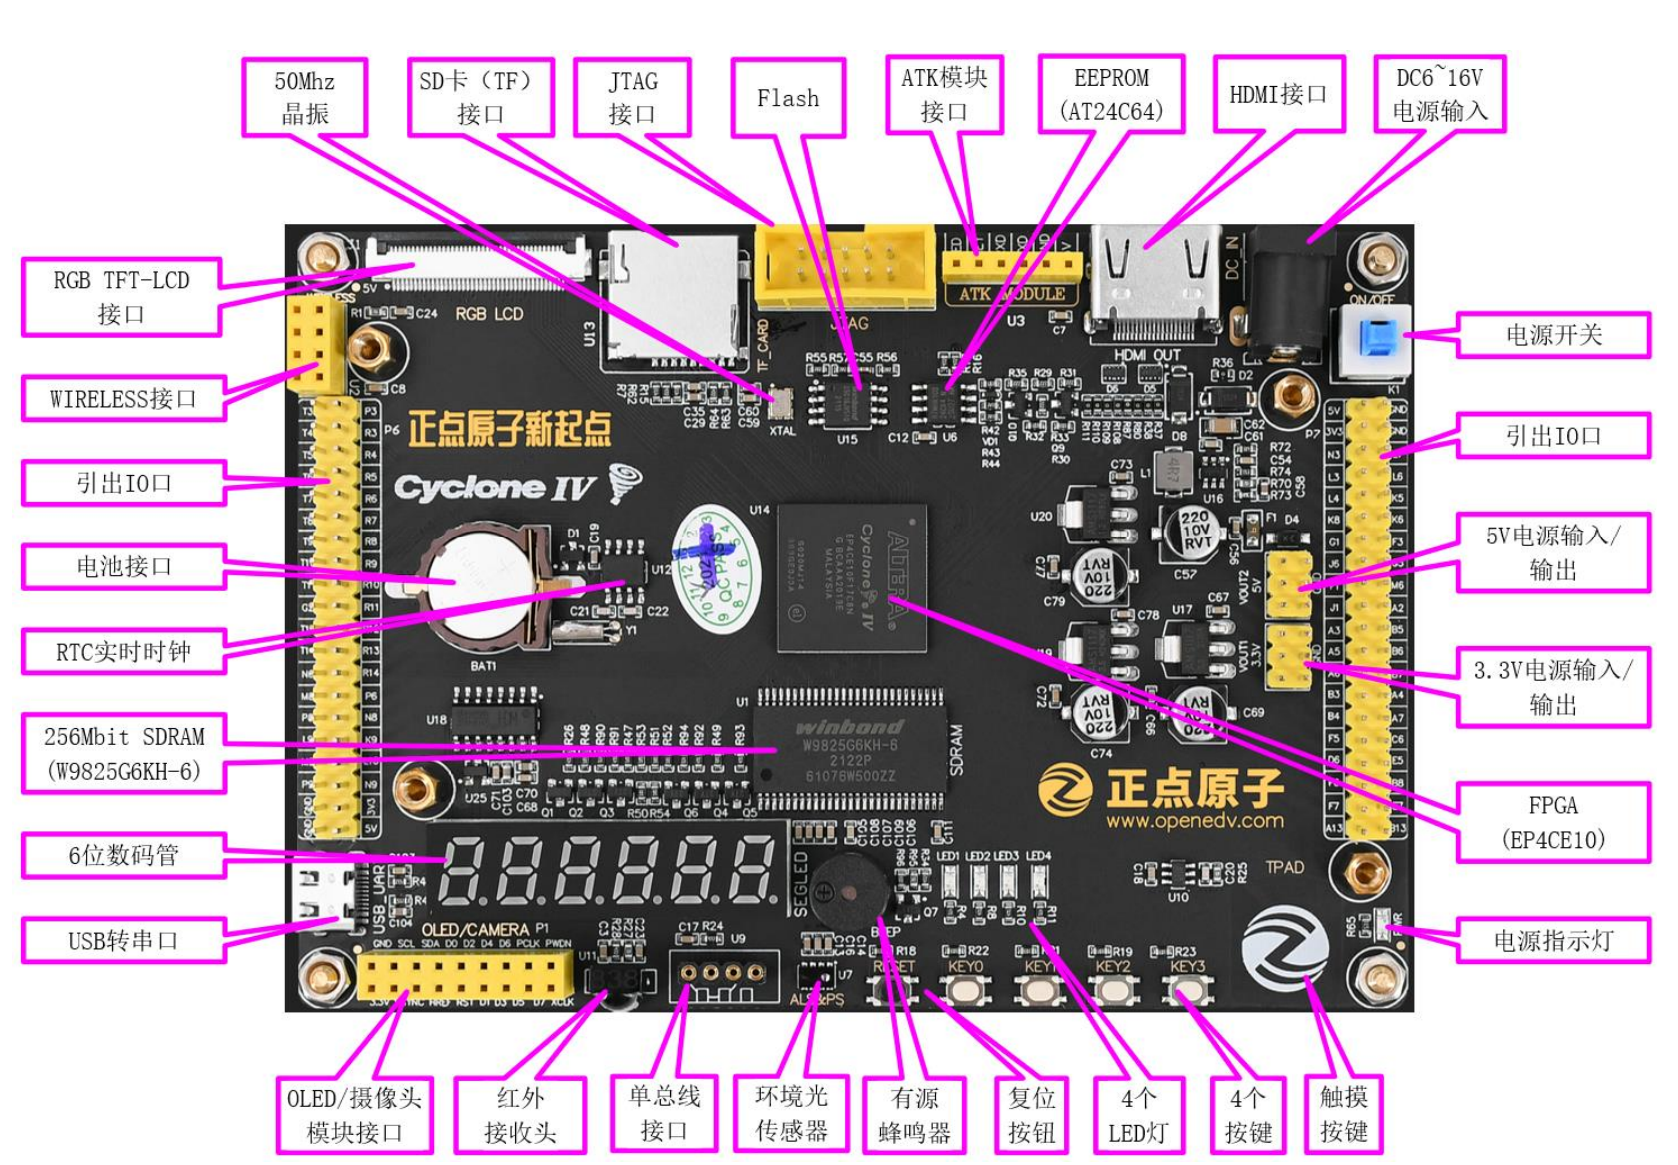
\includegraphics[width=0.8\textwidth]{FPGA.png}
    \caption{实验仪器与用具}
    \label{fig:实验仪器与用具}
\end{figure}

新起点 FPGA 开发板板载资源如下:

\begin{itemize}
    \item 主控芯片:EP4CE10F17C8N,封装:BGA256
    \item 晶振:50\,MHz
    \item FLASH:W25Q16,容量:16\,Mbit(2\,M字节)
    \item SDRAM:W9825G6KH-6,容量:256\,Mbit(32\,M字节)
    \item EEPROM:AT24C64,容量:64\,Kbit(8\,K字节)
    \item 1 个电源指示灯(蓝色)
    \item 4 个状态指示灯(DS0~DS3:红色)
    \item 1 个红外接收头,并配备一款小巧的红外遥控器
    \item 1 个无线模块接口,支持 NRF24L01 无线模块
    \item 1 路单总线接口,支持 DS18B20/DHT11 等单总线传感器
    \item 1 个 ATK 模块接口,支持正点原子蓝牙/GPS/MPU6050/RGB 灯模块
    \item 1 个环境光传感器,采用 AP3216C 芯片
    \item 1 个标准的 RGB TFT-LCD 接口
    \item 1 个 OLED/摄像头模块接口
    \item 1 个 USB 串口
    \item 1 个有源蜂鸣器
    \item 1 个 SD 卡接口(在板子背面)
    \item 1 个 HDMI 接口
    \item 1 个标准的 JTAG 调试下载口
    \item 1 组 5V 电源供应/接入口
    \item 1 组 3.3V 电源供应/接入口
    \item 1 个直流电源输入接口(输入电压范围:DC6~16V)
    \item 1 个 RTC 后备电池座,并带电池(在板子背面)
    \item 1 个 RTC 实时时钟,采用 PCF8563 芯片
    \item 1 个复位按钮,可作为 FPGA 程序执行的复位信号
    \item 4 个功能按钮
    \item 1 个电容触摸按键
    \item 1 个电源开关,控制整个开发板的电源
    \item 两个 20$\times$2 扩展口,共 72 个扩展 IO 口(除去电源和地)
\end{itemize}

\section{实验内容与步骤}
\subsection{概述}
\textbf{静态数码管显示实验}
\begin{enumerate}
\item[A.] 按照指南开发指南第十三章(P239)复现静态数码管显示实验,仿真部分暂时不用做
\item[B.] 修改原实验的按键逻辑,使其分别实现下述功能:
\item 将数字切换的时间间隔从0.5s改为0.25s,并固化程序到开发板中,实现断开下载器、电源后重启仍可实现LED流水灯(可通过修改MAX\_NUM实现)
\item 实现按键1控制时间间隔为0.5s,按键2控制时间间隔为0.25s(修改代码后还需要加入输入并分配引脚)
\end{enumerate}

\textbf{动态数码管显示实验}
\begin{enumerate}
\item[A.] 按照指南开发指南第十四章(P249)复现动态数码管显示实验,仿真部分暂时不用做
\item[B.] 修改原实验的按键逻辑,使其实现以下功能:
\item Key0可以暂停计数,key1可以改变计数加减模式(到0时不再减小),key2可以清零计数(主要修改count部分加减逻辑即可,需传入新输入并分配引脚)
\end{enumerate}

\cleardoublepage

\subsection{实验步骤}

\begin{enumerate}
    \item 新建 Project
    \begin{figure}[H]
        \centering
        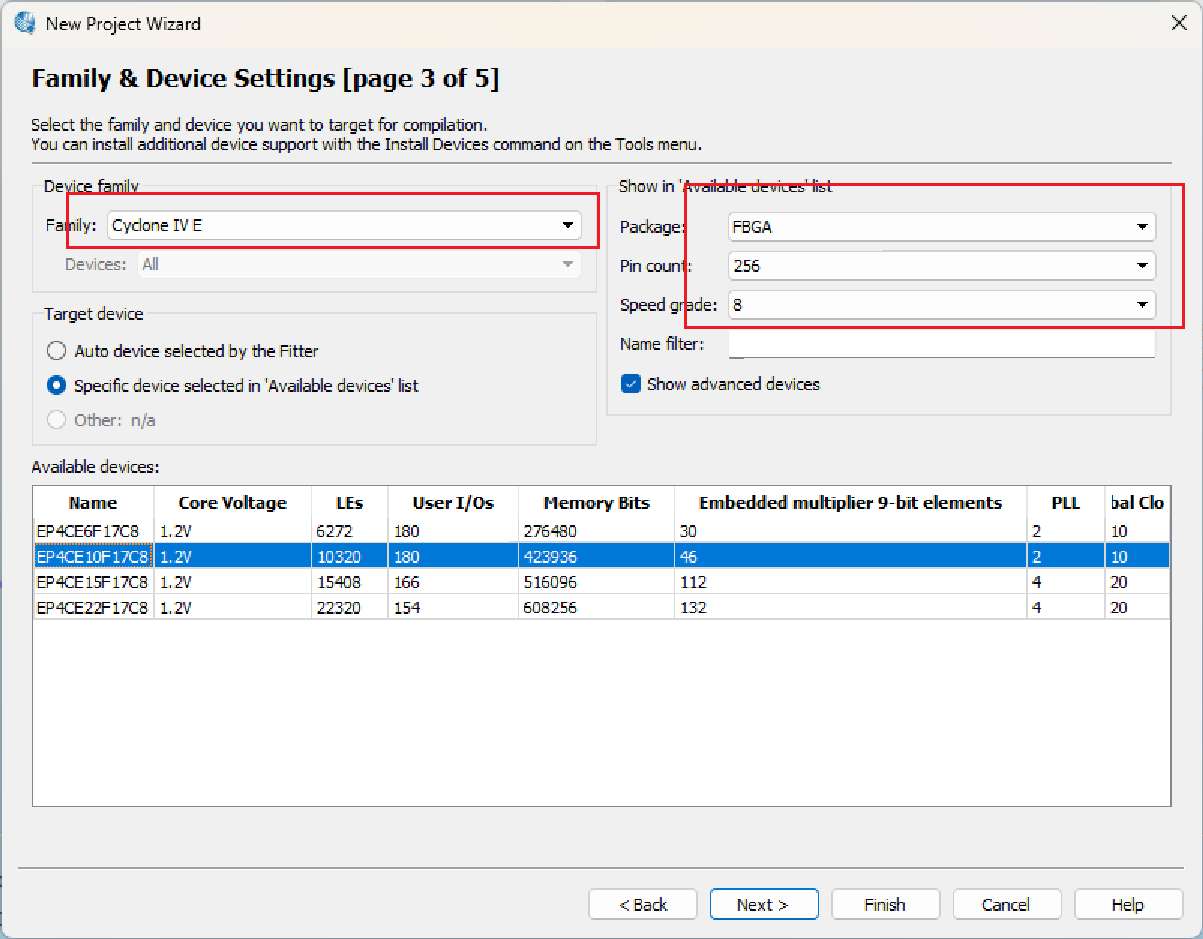
\includegraphics[width=0.7\textwidth]{step1.png}
        \caption{新建 Project 的操作界面1}
        \label{fig:step1}
    \end{figure}
    \begin{figure}[H]
        \centering
        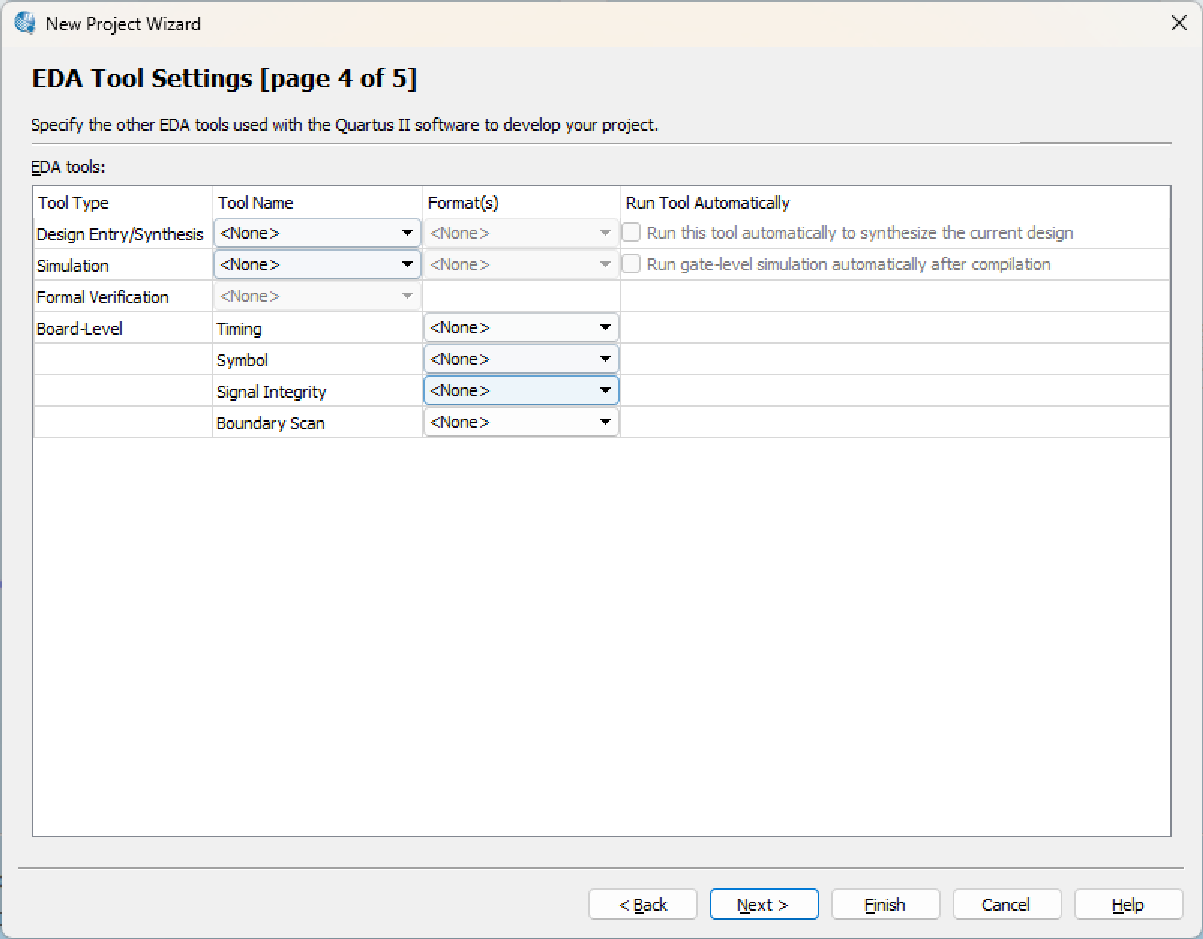
\includegraphics[width=0.7\textwidth]{step1_2.png}
        \caption{新建 Project 的操作界面2}
        \label{fig:step1_2}
    \end{figure}

\cleardoublepage

    \item 新建 .v 文件,编写代码并测试编译
    \begin{figure}[H]
        \centering
        \begin{subfigure}{0.3\textwidth}
            \centering
            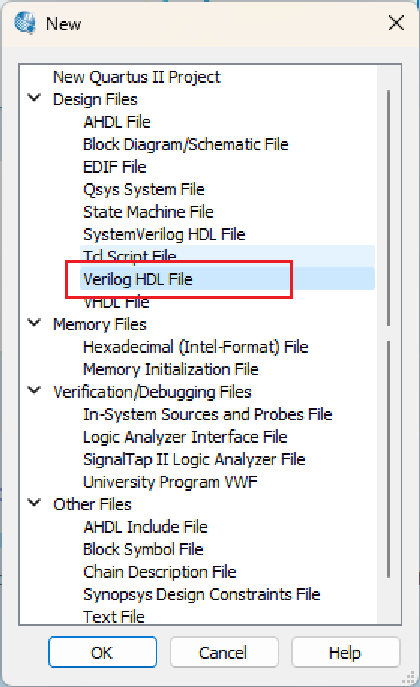
\includegraphics[width=\linewidth]{step2.png}
            \caption{新建 Verilog 文件}
            \label{fig:step2}
        \end{subfigure}
        \hfill
        \begin{subfigure}{0.68\textwidth}
            \centering
            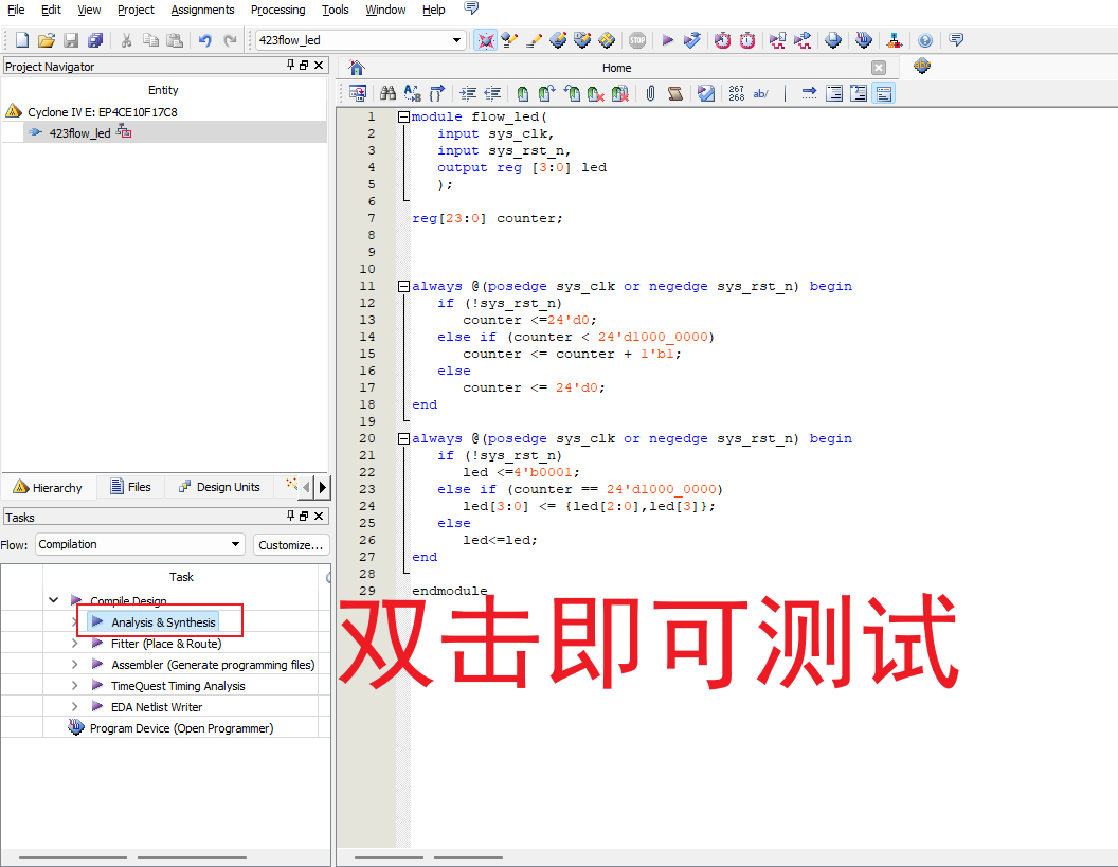
\includegraphics[width=\linewidth]{step2_2.png}
            \caption{代码编写界面}
            \label{fig:step2_2}
        \end{subfigure}
    \end{figure}
    \textbf{说明:}
    \begin{itemize}
        \item 在 Quartus 工程中新建 .v 文件后,双击打开文件,按照实验要求输入 Verilog 代码。
        \item 编写完成后,按 \textbf{Ctrl+S} 保存代码文件,确保文件已保存到 \textbf{rtl} 文件夹下,便于后续管理和调用。
        \item 保存后,右键点击该文件,选择“Add File to Project”,将代码文件添加到工程中。
        \item 在主界面点击“Analysis and Synthesis”或“Start Compilation”按钮,进行代码的语法检查和综合编译。
        \item 编译过程中如有语法错误,软件会在 Messages 窗口提示具体报错信息。根据提示修改代码,直至编译通过。
        \item 建议每次修改代码后都及时保存并重新编译,确保每一步更改都能被正确识别和验证。
    \end{itemize}
\cleardoublepage
    \item 预编译,确认无误
    \begin{figure}[H]
        \centering
        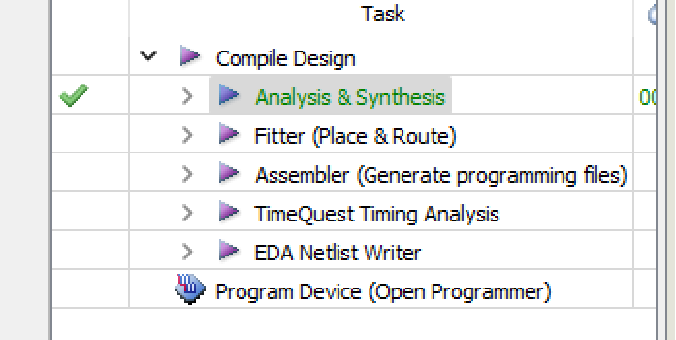
\includegraphics[width=0.7\textwidth]{step3.png}
        \caption{预编译结果界面1}
        \label{fig:step3}
    \end{figure}
    \begin{figure}[H]
        \centering
        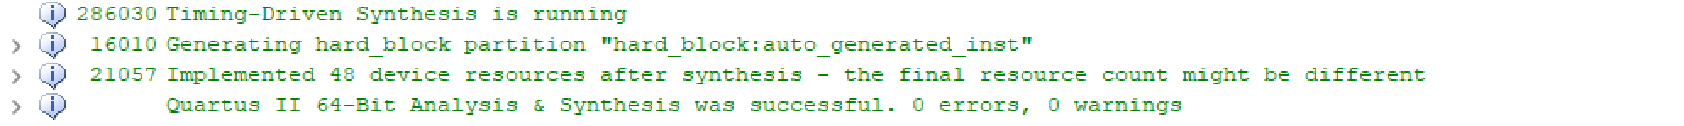
\includegraphics[width=0.7\textwidth]{step3_2.png}
        \caption{预编译结果界面2}
        \label{fig:step3_2}
    \end{figure}
    \textbf{说明:}预编译通过后,Quartus 的 Messages 窗口不会显示红色的 Error 报错信息,且 Analysis and Synthesis、Fitter 等阶段均能顺利完成。常见问题包括:代码语法错误、端口未连接、模块名或端口名拼写不一致、文件未正确添加到工程、顶层模块设置错误等。遇到报错时,可双击报错信息定位到具体代码行,根据提示逐一修改,直至所有错误消除。建议每次修改后都重新预编译,确保问题及时发现和解决。

\vspace{1cm}
    
    \item 注意 Project Name 和代码中的 module 名称一致
    \begin{figure}[H]
        \centering
        \begin{subfigure}{0.5\textwidth}
            \centering
            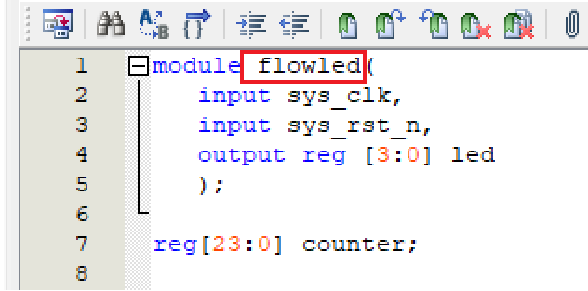
\includegraphics[width=\linewidth]{step4.png}
            \caption{Project Name}
            \label{fig:step4}
        \end{subfigure}
        \hfill
        \begin{subfigure}{0.45\textwidth}
            \centering
            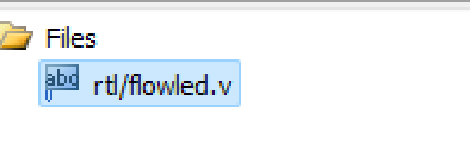
\includegraphics[width=\linewidth]{step4_2.png}
            \caption{module 名称}
            \label{fig:step4_2}
        \end{subfigure}
    \end{figure}
    \textbf{说明:}Project Name(工程名)和代码中的 module 名称保持一致,可以避免综合和仿真时出现顶层模块无法识别的问题。检查方法为:在新建工程时设置的 Project Name 应与顶层 Verilog 文件中的 module 名称完全相同(包括大小写),可通过工程属性和代码首行 module 语句进行核对。如不一致,建议修改工程名或 module 名称保持统一。
\cleardoublepage
    \item 保存代码文件至 rtl 文件夹内
    \begin{figure}[H]
        \centering
        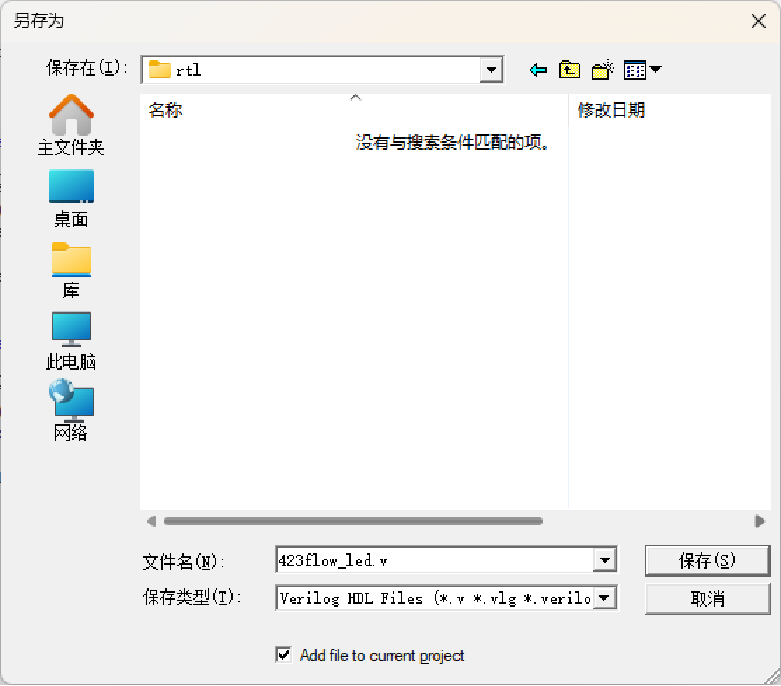
\includegraphics[width=0.7\textwidth]{step5.png}
        \caption{保存代码文件到指定文件夹}
        \label{fig:step5}
    \end{figure}
    \textbf{说明:}建议所有 Verilog 源代码文件统一保存在工程目录下的 \textbf{rtl} 文件夹内,便于管理和后续调用。图片文件建议存放于 \textbf{img} 文件夹,TCL 脚本等辅助文件可放在 \textbf{script} 文件夹。文件命名应简洁明了,避免使用中文、空格或特殊字符,推荐使用小写字母、数字和下划线组合。例如:\texttt{seg\_led\_static.v}、\texttt{step1.png}。这样有助于工程的规范化管理和后期维护。

\cleardoublepage

    \item 打开 Pin Planner 分配引脚
    \begin{figure}[H]
        \centering
        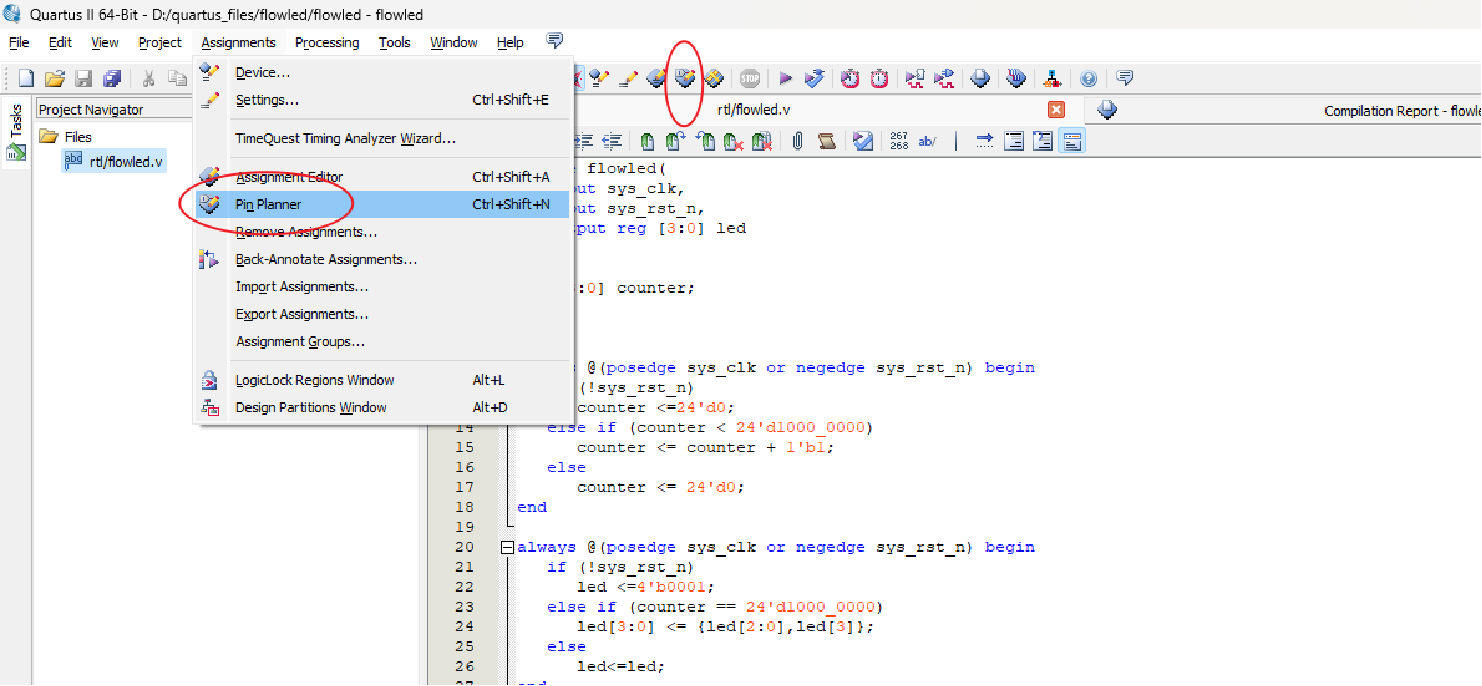
\includegraphics[width=0.8\textwidth]{step6.png}
        \caption{Pin Planner 分配引脚界面}
        \label{fig:step6}
    \end{figure}
    \textbf{说明:}在 Quartus 中分配引脚时,首先点击工具栏的“Assignments”菜单,选择“Pin Planner”进入引脚分配界面。根据原理图或实验指导书,将各个信号(如时钟、复位、数码管段选、位选、按键等)对应到实际开发板的物理引脚编号。在 Pin Planner 界面左侧找到信号名称,右侧输入或选择对应的引脚编号。分配完成后,点击保存并关闭 Pin Planner。建议分配完引脚后进行一次完整编译,确保无引脚冲突或未分配等错误。如有 tcl 脚本文件,也可通过“Assignments”→“Import Assignments”导入脚本自动分配引脚。
\cleardoublepage

    \item 手动输入/使用 tcl 脚本文件
    \begin{figure}[H]
        \centering
        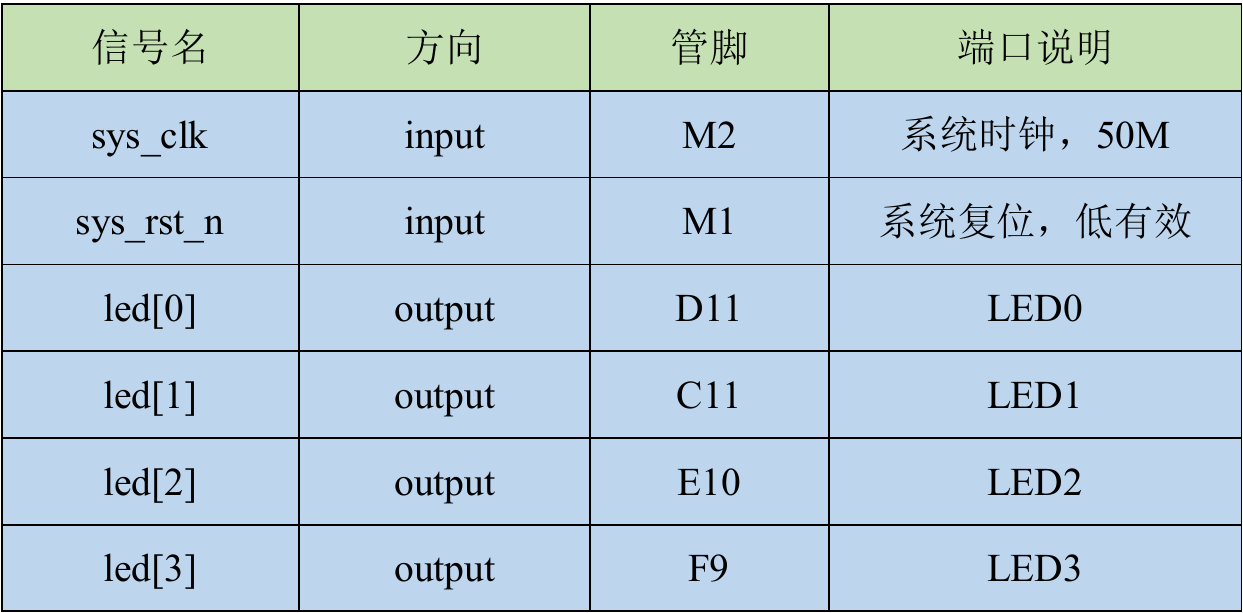
\includegraphics[width=0.7\textwidth]{step7.png}
        \caption{tcl 脚本分配引脚示意}
        \label{fig:step7}
    \end{figure}
    \textbf{tcl 脚本示例:}
    \begin{lstlisting}[language=Matlab, style=MatlabStyle_src]
        set_location_assignment PIN_M2 -to sys_clk
        set_location_assignment PIN_M1 -to sys_rst_n
        set_location_assignment PIN_D11 -to led[0]
        set_location_assignment PIN_C11 -to led[1]
        set_location_assignment PIN_E10 -to led[2]
        set_location_assignment PIN_F9 -to led[3]
    \end{lstlisting}
    \textbf{说明:}手动分配引脚适合引脚数量较少或仅需少量调整的情况,操作直观,可直接在 Pin Planner 图形界面中完成,便于初学者理解和检查。使用 tcl 脚本分配引脚则适合引脚较多或需多次复用、批量管理的场景,只需准备好脚本文件即可一键导入,效率更高,也便于团队协作和版本管理。实际操作时,建议在项目初期用 Pin Planner 熟悉引脚分配流程,后续可通过 tcl 脚本实现自动化和规范化管理。
  
\cleardoublepage    
    
    \item 完整编译工程
    \begin{figure}[H]
        \centering
        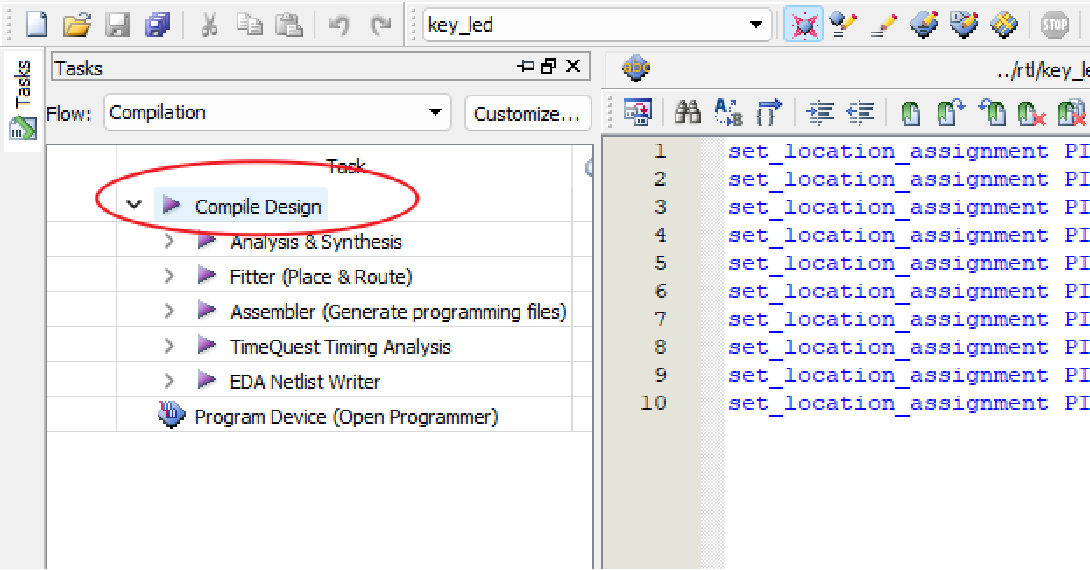
\includegraphics[width=0.7\textwidth]{step8.png}
        \caption{完整编译工程界面}
        \label{fig:step8}
    \end{figure}
    \textbf{说明:}完整编译流程包括:首先点击主界面的“Start Compilation”按钮,Quartus 会自动依次执行 Analysis \& Synthesis、Fitter、Assembler、TimeQuest Timing Analysis 等步骤。编译过程中如遇到错误(Error)或警告(Warning),可在 Messages 窗口查看详细信息,双击可定位到相关代码或设置。常见注意事项包括:确保所有源文件已正确添加到工程、顶层模块设置无误、引脚分配无冲突、时钟约束合理等。建议每次修改代码或引脚分配后都重新完整编译,确保设计的正确性和可用性。
\cleardoublepage

    \item 下载程序至开发板
    \begin{figure}[H]
        \centering
        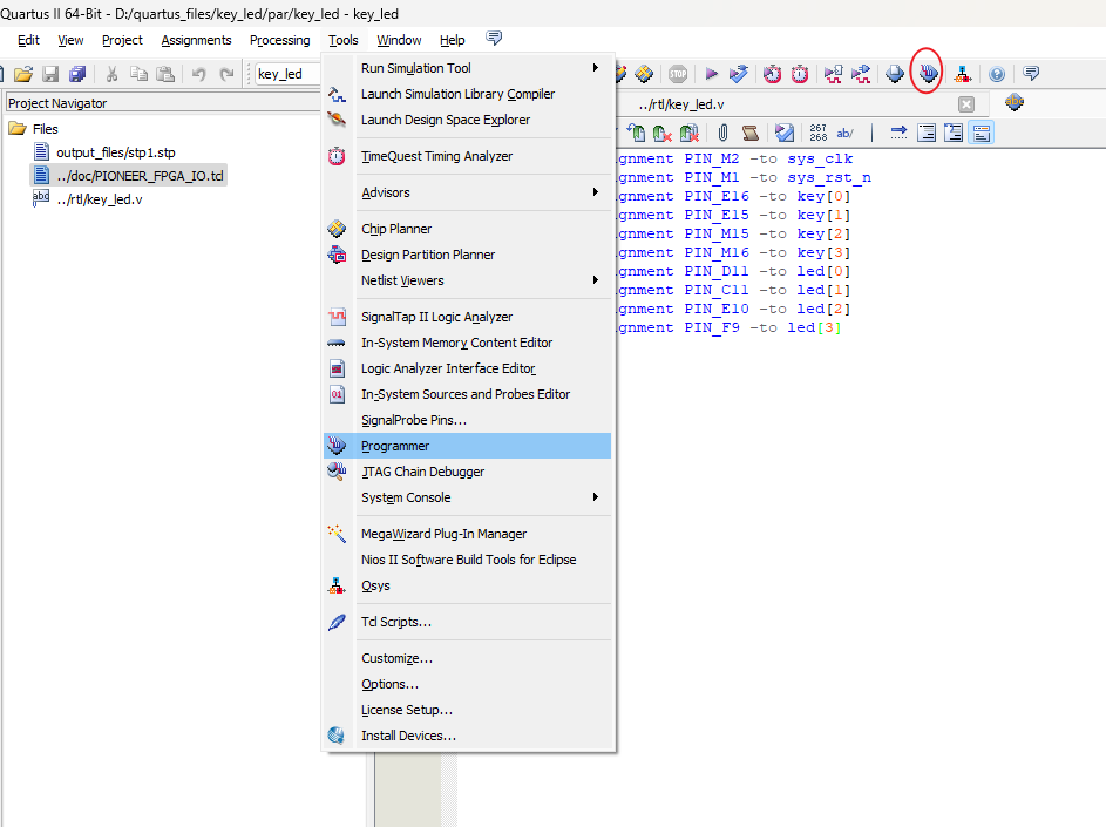
\includegraphics[width=0.7\textwidth]{step9.png}
        \caption{下载程序到开发板界面1}
        \label{fig:step9}
    \end{figure}

    \begin{figure}[H]
        \centering
        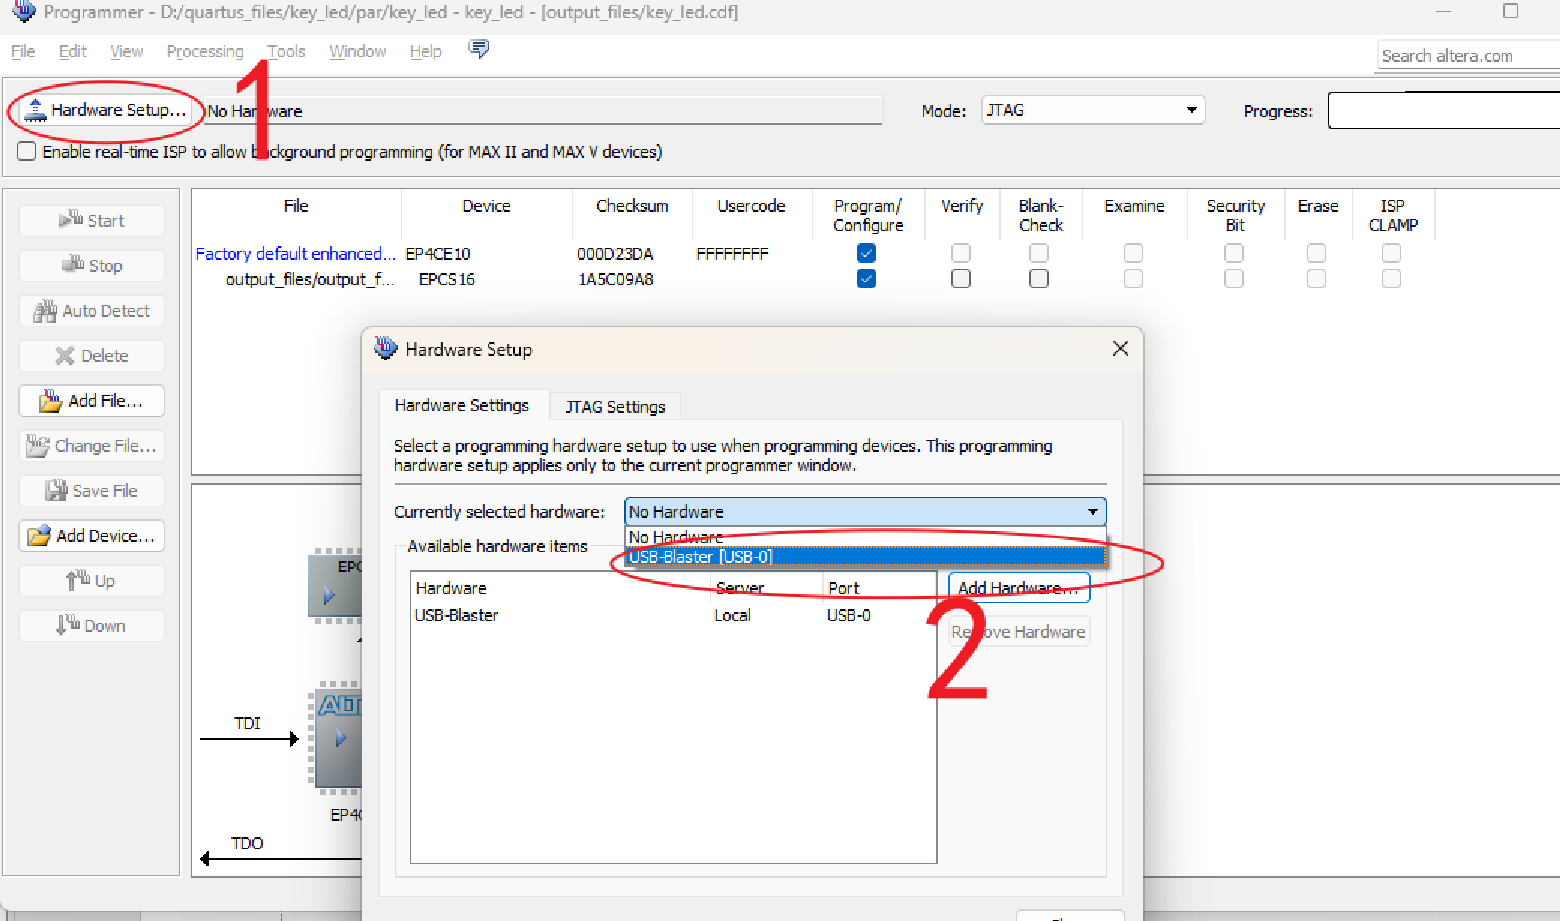
\includegraphics[width=0.7\textwidth]{step9_2.png}
        \caption{下载程序到开发板界面2}
        \label{fig:step9_2}
    \end{figure}

    \begin{figure}[H]
        \centering
        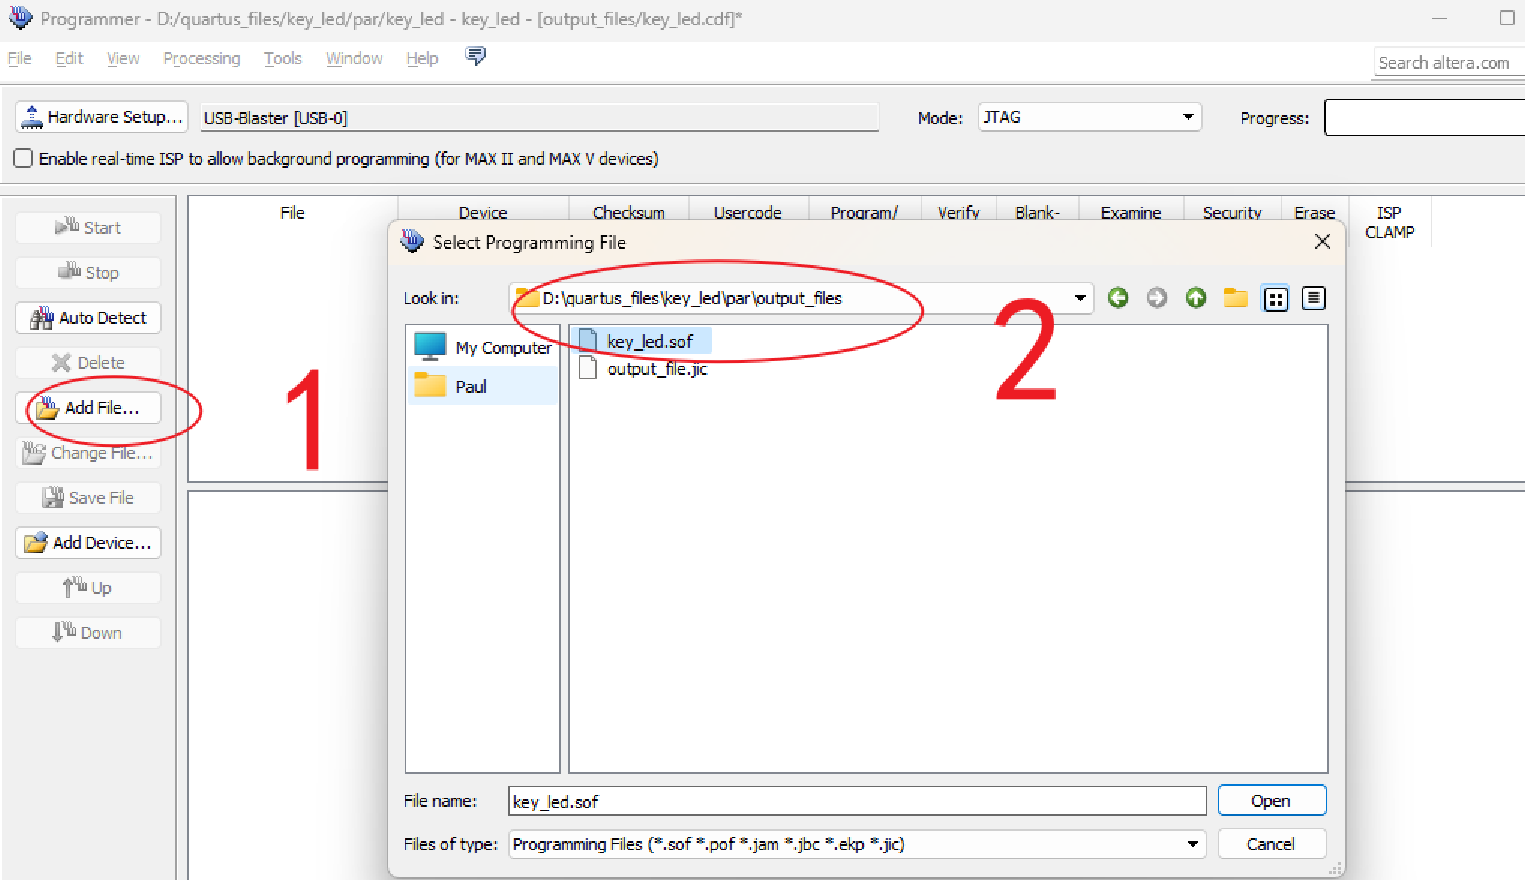
\includegraphics[width=0.7\textwidth]{step9_3.png}
        \caption{下载程序到开发板界面3}
        \label{fig:step9_3}
    \end{figure}

    \begin{figure}[H]
        \centering
        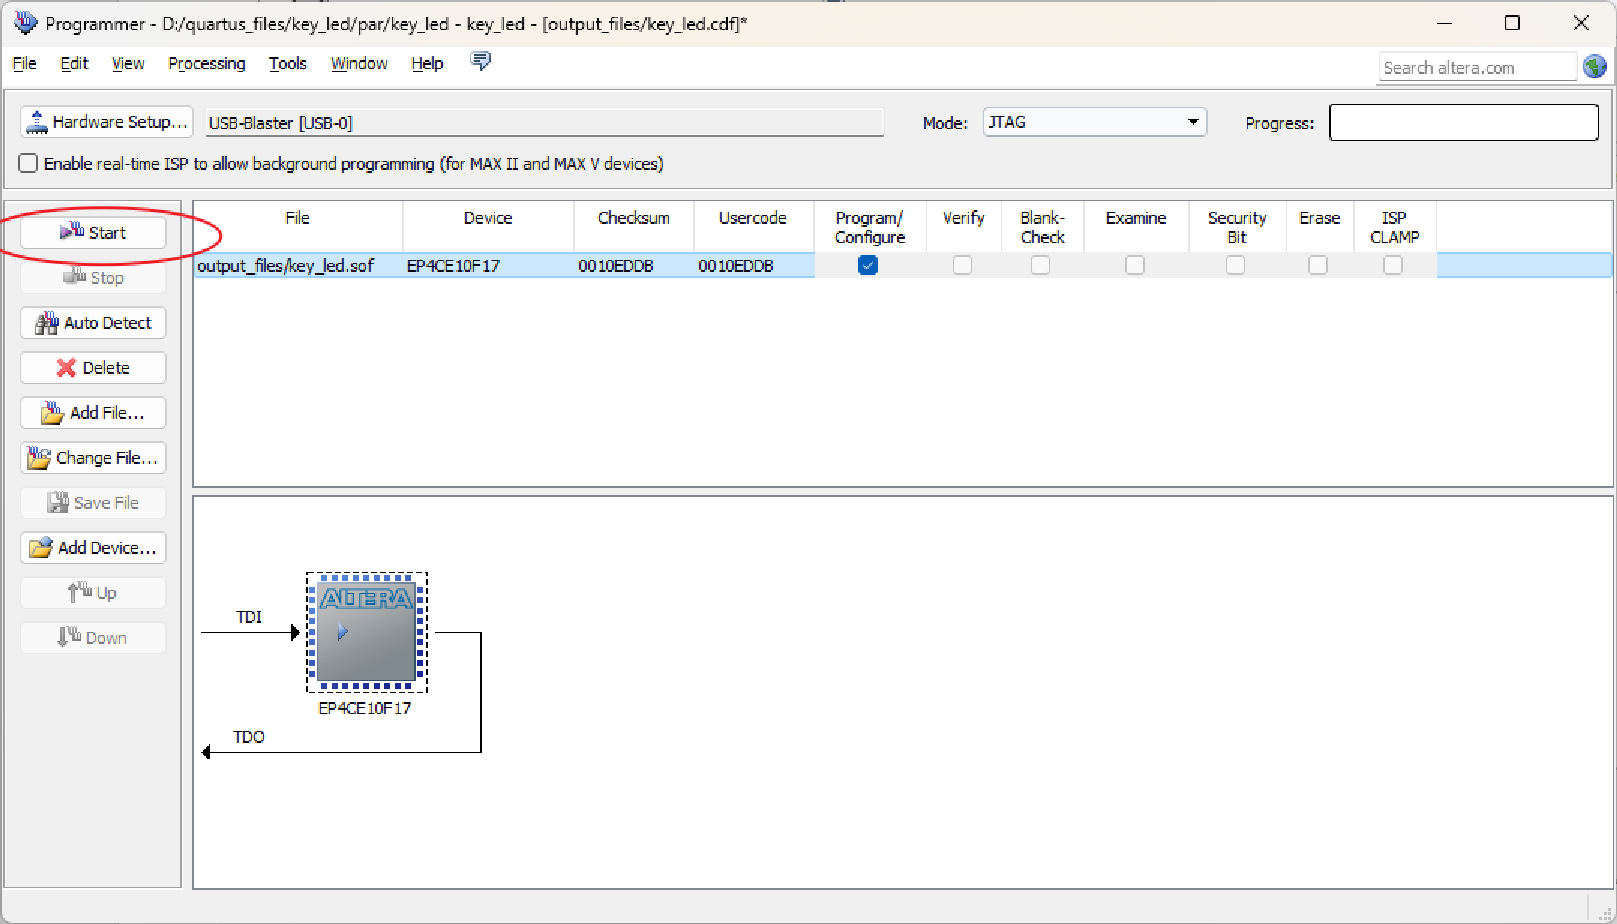
\includegraphics[width=0.7\textwidth]{step9_4.png}
        \caption{下载程序到开发板界面4}
        \label{fig:step9_4}
    \end{figure}
    \textbf{说明:}下载程序到开发板的步骤如下:首先确保开发板已正确连接至电脑,并安装好驱动程序。打开 Quartus,点击工具栏的“Programmer”按钮,进入下载界面。点击“Hardware Setup”选择正确的下载器型号(如 USB-Blaster),然后点击“Auto Detect”自动识别芯片。添加编译生成的 .sof 文件,勾选“Program/Configure”,最后点击“Start”按钮开始下载。下载完成后,观察开发板上的数码管显示是否正常。常见问题包括:未识别到下载器、芯片型号选择错误、下载过程中断等,遇到问题可尝试重新连接设备、检查驱动或重启软件。
\cleardoublepage
    \item 导出 jic 文件,固化程序
    \begin{figure}[H]
        \centering
        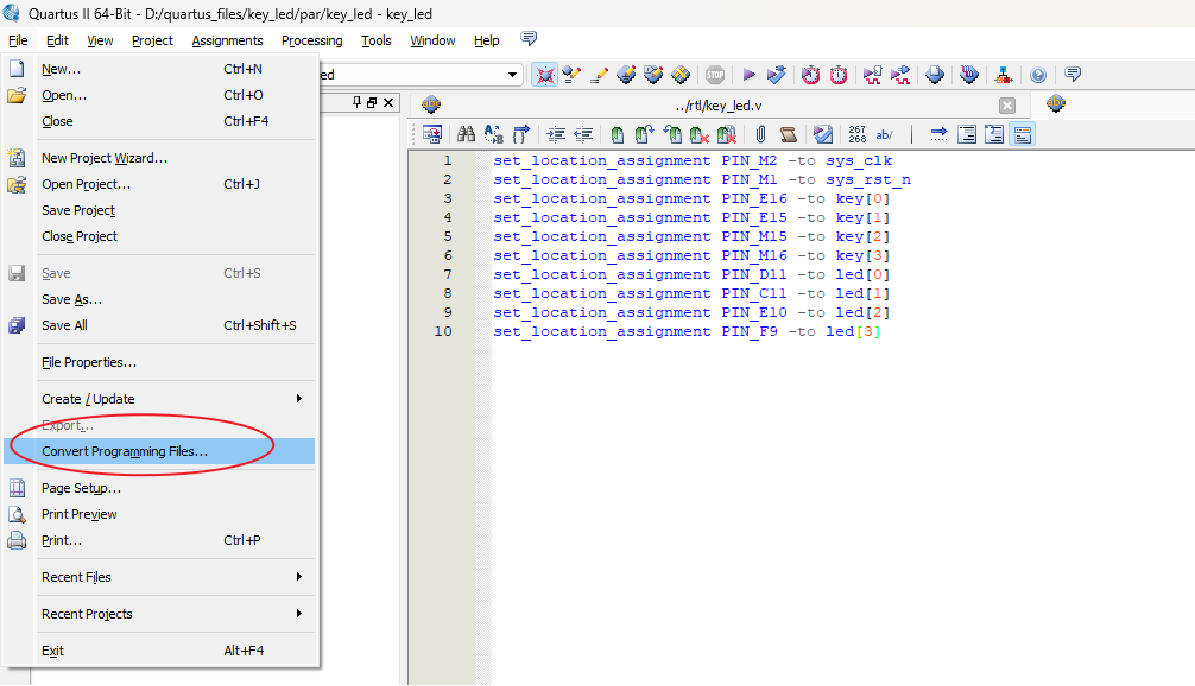
\includegraphics[width=0.7\textwidth]{step10.png}
        \caption{导出 jic 文件界面}
        \label{fig:step10}
    \end{figure}

    \begin{figure}[H]
        \centering
        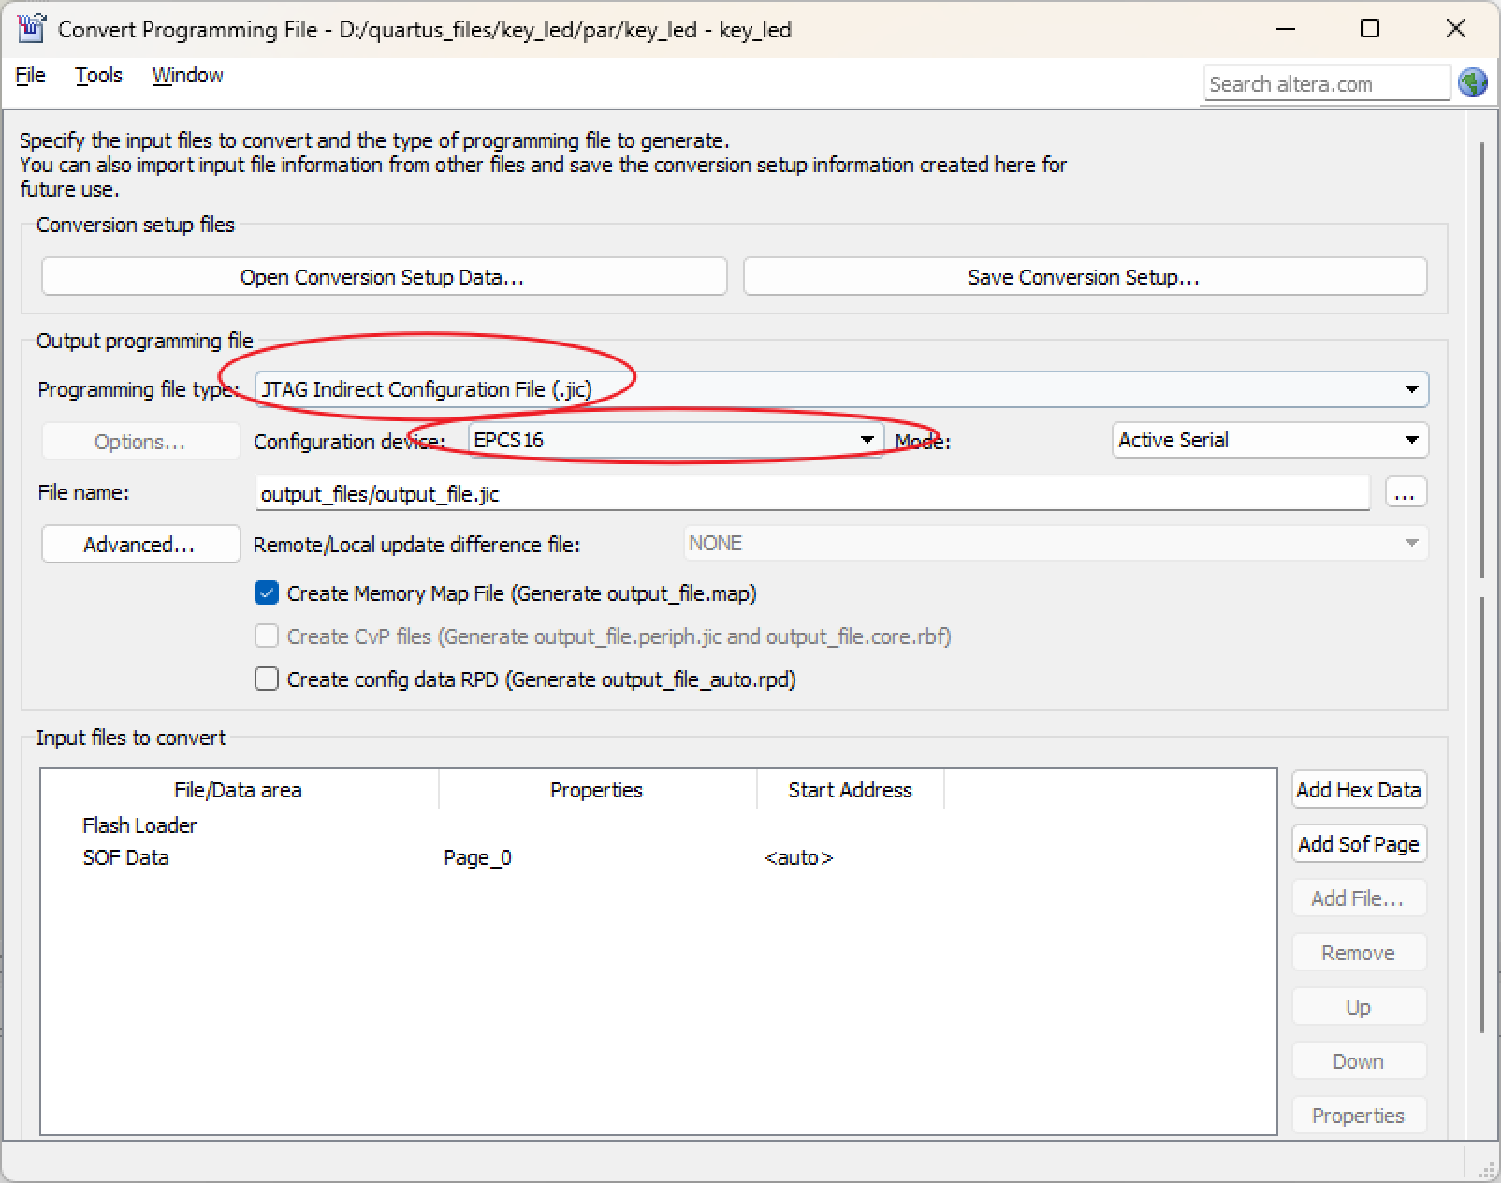
\includegraphics[width=0.7\textwidth]{step10_2.png}
        \caption{导出 jic 文件界面2}
        \label{fig:step10_2}
    \end{figure}

    \begin{figure}[H]
        \centering
        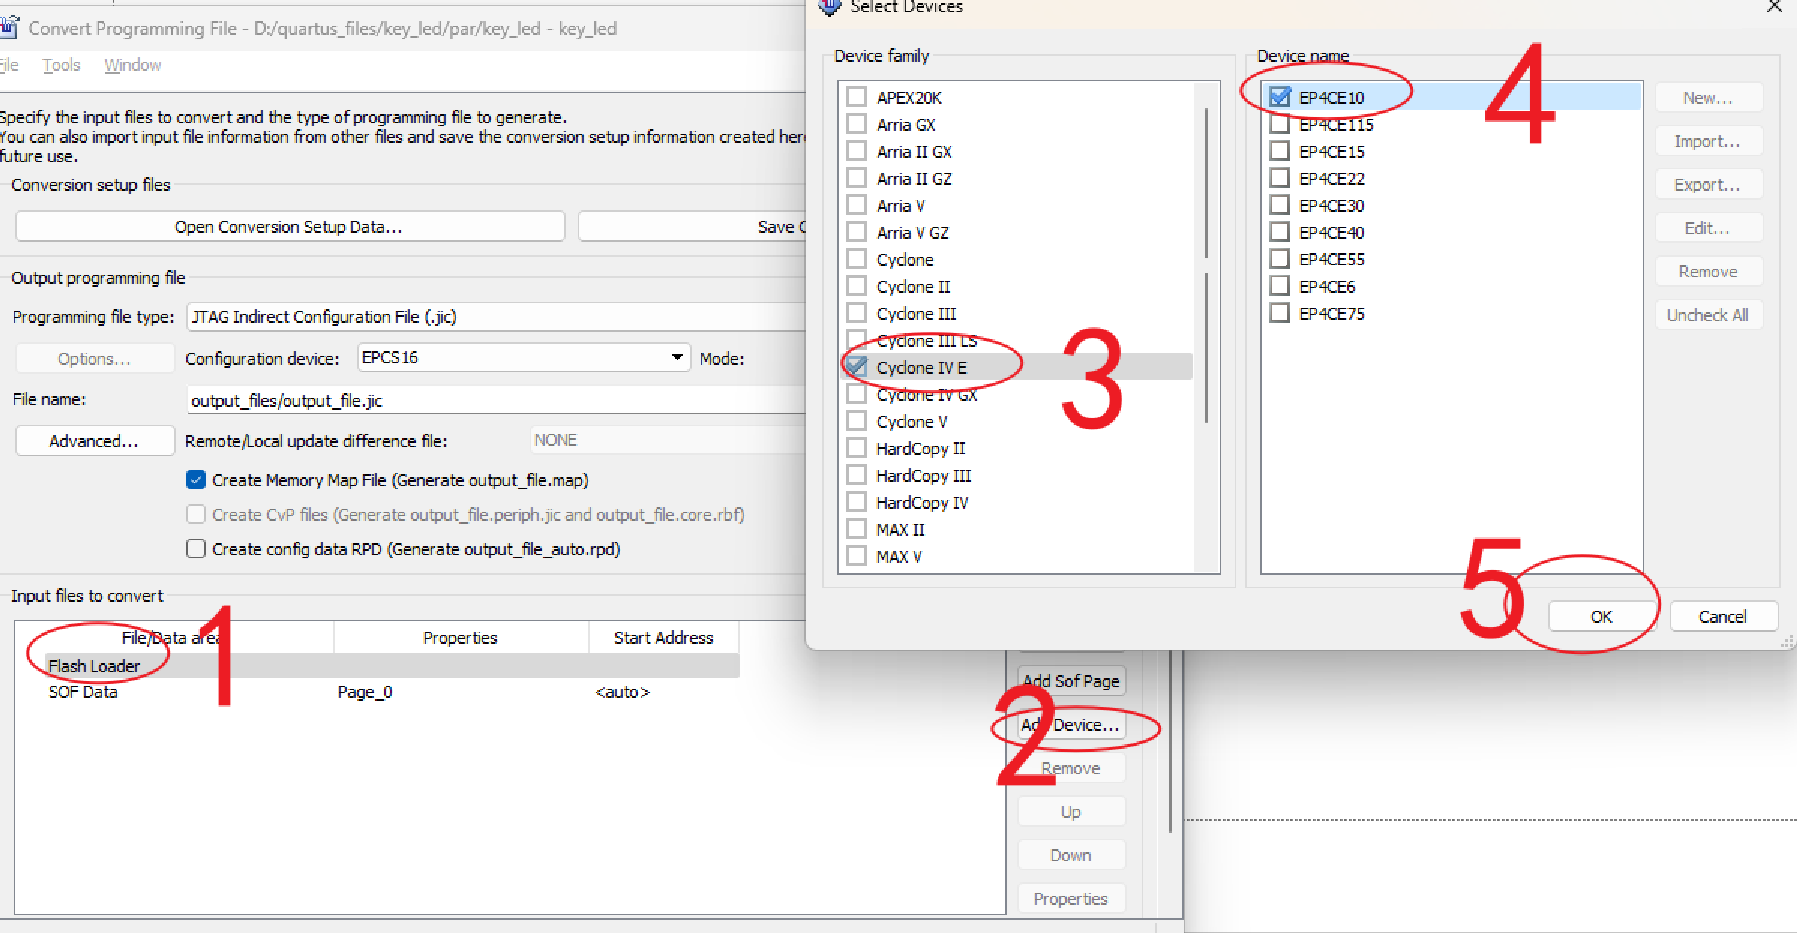
\includegraphics[width=0.7\textwidth]{step10_3.png}
        \caption{导出 jic 文件界面3}
        \label{fig:step10_3}
    \end{figure}

    \begin{figure}[H]
        \centering
        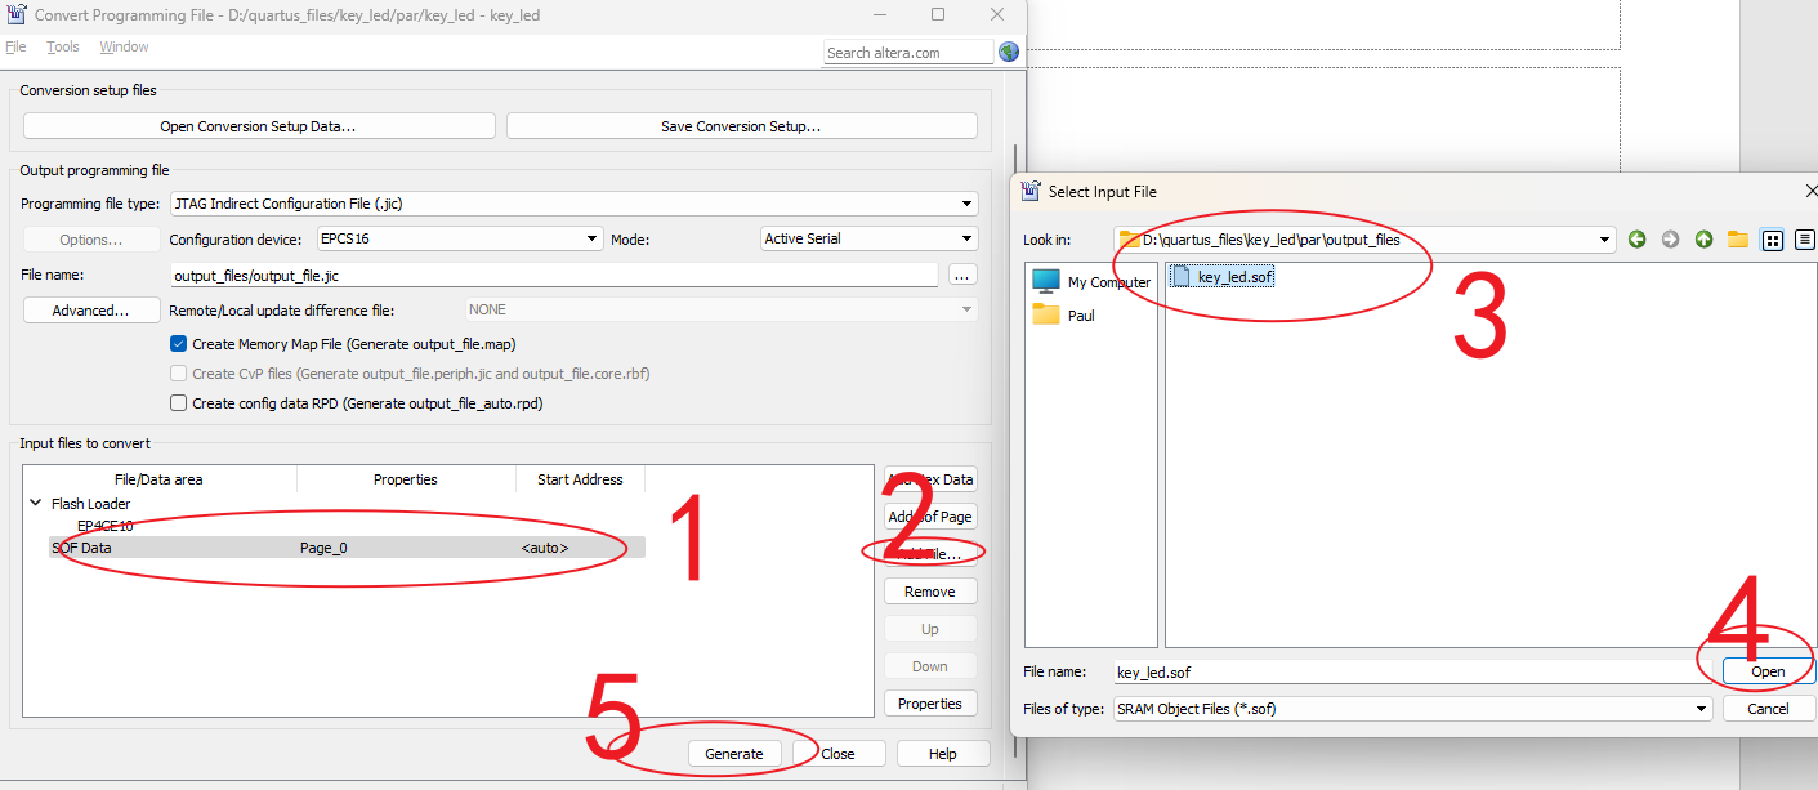
\includegraphics[width=0.7\textwidth]{step10_4.png}
        \caption{导出 jic 文件界面4}
        \label{fig:step10_4}
    \end{figure}

    \textbf{说明:}固化流程如下:首先在 Quartus 中点击“File”菜单,选择“Convert Programming Files”,在弹出的窗口中将 File Type 选择为 JTAG Indirect Configuration File(.jic),并选择对应的目标器件和 Flash 类型。添加已编译生成的 .sof 文件,设置输出文件名和路径,点击“Generate”生成 .jic 文件。生成后,打开“Programmer”界面,将 Mode 设置为“Active Serial Programming”,添加 .jic 文件,选择目标 Flash 芯片,勾选“Program/Configure”,点击“Start”开始固化。固化完成后,断电重启开发板,程序即可自动运行。注意事项:固化前确保芯片型号和 Flash 类型选择正确,避免误操作导致固化失败;固化过程中请勿断开电源或数据线;如遇固化失败,可尝试重新生成 .jic 文件或检查硬件连接。
\end{enumerate}




\cleardoublepage

\section{实验结果}

\subsection{实验结果1:静态数码管显示实验基础问题}
\noindent
\textbf{演示视频:}\href{https://www.bilibili.com/video/BV18iVRzWEar?vd_source=4fd6c4265e65c0785c912874692a3971}{点击查看演示视频}

\subsection{实验结果2:静态数码管显示实验变式1}
\noindent
\textbf{演示视频:}\href{https://www.bilibili.com/video/BV1zJVRzNEHS?vd_source=4fd6c4265e65c0785c912874692a3971}{点击查看演示视频}

\subsection{实验结果3:静态数码管显示实验变式2}
\noindent
\textbf{演示视频:}\href{https://www.bilibili.com/video/BV1t6VRzDEVM?vd_source=4fd6c4265e65c0785c912874692a3971}{点击查看演示视频}

\subsection{实验结果4:动态数码管显示实验基础问题}
\noindent
\textbf{演示视频:}\href{https://www.bilibili.com/video/BV1u6VRzQE7A?vd_source=4fd6c4265e65c0785c912874692a3971}{点击查看演示视频}

\subsection{实验结果5:动态数码管显示实验变式}
\noindent
\textbf{演示视频:}\href{https://www.bilibili.com/video/BV1t6VRzDEs3?vd_source=4fd6c4265e65c0785c912874692a3971}{点击查看演示视频}

\section{实验总结}

\subsection{实验中的问题与感想}

\begin{enumerate}
\item 在这次实验过程中,由于助教老师已经给出了TCL脚本文件,所以我们只需要在代码中添加引脚分配即可,节省了不少时间。
\item 但不得不提的是,之前我们实验中使用的手动分配引脚,现在采取导入TCL文件,对于我们来说是一个新的挑战。因为我们需要在代码中添加引脚分配,而不是在图形化界面中进行操作。
\item 这次实验中,我们还需要对按键的逻辑进行修改,这也是一个挑战。我们需要仔细阅读代码,理解每一行的含义,并进行相应的修改。
\item 这次还有一个问题,在给出的代码和引脚TCL文件中出现了冲突,原因是sel和seg\_sel不同的命名方式导致了运行冲突。
\item 另外,实验中还需要注意的是,按键的逻辑需要根据实际情况进行修改,比如按键的时间间隔、计数加减模式等,这些都需要我们仔细考虑。
\end{enumerate}

\cleardoublepage
\section{附录:Verilog 代码}

\textbf{Verilog 代码:静态数码管显示实验基础问题}
\begin{lstlisting}[language=Matlab, style=MatlabStyle_src]
module seg_led_static_top (
    input               sys_clk  ,       // 系统时钟
    input               sys_rst_n,       // 系统复位信号(低有效)

    output    [5:0]     seg_sel  ,       // 数码管位选
    output    [7:0]     seg_led          // 数码管段选

);

//parameter define
parameter  TIME_SHOW = 25'd25000_000;    // 数码管变化的时间间隔0.5s

//wire define
wire       add_flag;                     // 数码管变化的通知信号

//*****************************************************
//**                    main code
//*****************************************************

//每隔0.5s产生一个时钟周期的脉冲信号
time_count #(
    .MAX_NUM    (TIME_SHOW)
) u_time_count(
    .clk        (sys_clk  ),
    .rst_n      (sys_rst_n),
    
    .flag       (add_flag )
);

//每当脉冲信号到达时,使数码管显示的数值加1
seg_led_static u_seg_led_static (
    .clk        (sys_clk  ), 
    .rst_n      (sys_rst_n),

    .add_flag   (add_flag ), 
    .seg_sel    (seg_sel  ),
    .seg_led    (seg_led  )
);

endmodule 


module time_count(
    input           clk     ,   // 时钟信号
    input           rst_n   ,   // 复位信号

    output   reg    flag        // 一个时钟周期的脉冲信号
);

//parameter define
parameter  MAX_NUM = 25000_000; // 计数器最大计数值

//reg define
reg [24:0] cnt;                 // 时钟分频计数器

//*****************************************************
//**                    main code
//*****************************************************

//计数器对时钟计数,每计时到0.5s,输出一个时钟周期的脉冲信号
always @ (posedge clk or negedge rst_n) begin
    if (!rst_n) begin
        flag <= 1'b0;
        cnt  <= 24'b0;
    end
    else if(cnt < MAX_NUM - 1'b1) begin
        cnt  <= cnt +1'b1;
        flag <= 1'b0;
    end
    else begin
        cnt  <= 24'b0;
        flag <= 1'b1;
    end
end

endmodule 


module seg_led_static (
    input               clk     ,   // 时钟信号
    input               rst_n   ,   // 复位信号(低有效)

    input               add_flag,   // 数码管变化的通知信号
    output  reg  [5:0]  seg_sel ,   // 数码管位选
    output  reg  [7:0]  seg_led     // 数码管段选
);

//reg define
reg [3:0] num;                      // 数码管显示的十六进制数

//*****************************************************
//**                    main code
//*****************************************************

//控制数码管位选信号(低电平有效),选中所有的数码管
always @ (posedge clk or negedge rst_n) begin
    if (!rst_n)
        seg_sel <= 6'b111111;
    else
        seg_sel <= 6'b000000;
end

//每次通知信号到达时,数码管显示的十六进制数值加1
always @ (posedge clk or negedge rst_n) begin
    if (!rst_n)
        num <= 4'h0;
    else if(add_flag) begin
        if (num < 4'hf)
            num <= num + 1'b1;
        else
            num <= 4'h0;
    end
    else
        num <= num;
end

//根据数码管显示的数值,控制段选信号
always @ (posedge clk or negedge rst_n) begin
    if (!rst_n)
        seg_led <= 8'b0;
    else begin
        case (num)
            4'h0 :    seg_led <= 8'b1100_0000;
            4'h1 :    seg_led <= 8'b1111_1001;
            4'h2 :    seg_led <= 8'b1010_0100;
            4'h3 :    seg_led <= 8'b1011_0000;
            4'h4 :    seg_led <= 8'b1001_1001;
            4'h5 :    seg_led <= 8'b1001_0010;
            4'h6 :    seg_led <= 8'b1000_0010;
            4'h7 :    seg_led <= 8'b1111_1000;
            4'h8 :    seg_led <= 8'b1000_0000;
            4'h9 :    seg_led <= 8'b1001_0000;
            4'ha :    seg_led <= 8'b1000_1000;
            4'hb :    seg_led <= 8'b1000_0011;
            4'hc :    seg_led <= 8'b1100_0110;
            4'hd :    seg_led <= 8'b1010_0001;
            4'he :    seg_led <= 8'b1000_0110;
            4'hf :    seg_led <= 8'b1000_1110;
            default : seg_led <= 8'b1100_0000;
        endcase
    end
end

endmodule 

\end{lstlisting}


\cleardoublepage

\textbf{Verilog 代码:静态数码管显示实验变式1}
\begin{lstlisting}[language=Matlab, style=MatlabStyle_src]
module seg_led_static_top_acc (
    input               sys_clk  ,       // 系统时钟
    input               sys_rst_n,       // 系统复位信号(低有效)

    output    [5:0]     seg_sel  ,       // 数码管位选
    output    [7:0]     seg_led          // 数码管段选

);

//parameter define
parameter  TIME_SHOW = 25'd12500_000;    // 数码管变化的时间间隔0.5s

//wire define
wire       add_flag;                     // 数码管变化的通知信号

//*****************************************************
//**                    main code
//*****************************************************

//每隔0.5s产生一个时钟周期的脉冲信号
time_count #(
    .MAX_NUM    (TIME_SHOW)
) u_time_count(
    .clk        (sys_clk  ),
    .rst_n      (sys_rst_n),
    
    .flag       (add_flag )
);

//每当脉冲信号到达时,使数码管显示的数值加1
seg_led_static u_seg_led_static (
    .clk        (sys_clk  ), 
    .rst_n      (sys_rst_n),

    .add_flag   (add_flag ), 
    .seg_sel    (seg_sel  ),
    .seg_led    (seg_led  )
);

endmodule 


module time_count(
    input           clk     ,   // 时钟信号
    input           rst_n   ,   // 复位信号

    output   reg    flag        // 一个时钟周期的脉冲信号
);

//parameter define
parameter  MAX_NUM = 12500_000; // 计数器最大计数值

//reg define
reg [24:0] cnt;                 // 时钟分频计数器

//*****************************************************
//**                    main code
//*****************************************************

//计数器对时钟计数,每计时到0.5s,输出一个时钟周期的脉冲信号
always @ (posedge clk or negedge rst_n) begin
    if (!rst_n) begin
        flag <= 1'b0;
        cnt  <= 24'b0;
    end
    else if(cnt < MAX_NUM - 1'b1) begin
        cnt  <= cnt +1'b1;
        flag <= 1'b0;
    end
    else begin
        cnt  <= 24'b0;
        flag <= 1'b1;
    end
end

endmodule 


module seg_led_static (
    input               clk     ,   // 时钟信号
    input               rst_n   ,   // 复位信号(低有效)

    input               add_flag,   // 数码管变化的通知信号
    output  reg  [5:0]  seg_sel ,   // 数码管位选
    output  reg  [7:0]  seg_led     // 数码管段选
);

//reg define
reg [3:0] num;                      // 数码管显示的十六进制数

//*****************************************************
//**                    main code
//*****************************************************

//控制数码管位选信号(低电平有效),选中所有的数码管
always @ (posedge clk or negedge rst_n) begin
    if (!rst_n)
        seg_sel <= 6'b111111;
    else
        seg_sel <= 6'b000000;
end

//每次通知信号到达时,数码管显示的十六进制数值加1
always @ (posedge clk or negedge rst_n) begin
    if (!rst_n)
        num <= 4'h0;
    else if(add_flag) begin
        if (num < 4'hf)
            num <= num + 1'b1;
        else
            num <= 4'h0;
    end
    else
        num <= num;
end

//根据数码管显示的数值,控制段选信号
always @ (posedge clk or negedge rst_n) begin
    if (!rst_n)
        seg_led <= 8'b0;
    else begin
        case (num)
            4'h0 :    seg_led <= 8'b1100_0000;
            4'h1 :    seg_led <= 8'b1111_1001;
            4'h2 :    seg_led <= 8'b1010_0100;
            4'h3 :    seg_led <= 8'b1011_0000;
            4'h4 :    seg_led <= 8'b1001_1001;
            4'h5 :    seg_led <= 8'b1001_0010;
            4'h6 :    seg_led <= 8'b1000_0010;
            4'h7 :    seg_led <= 8'b1111_1000;
            4'h8 :    seg_led <= 8'b1000_0000;
            4'h9 :    seg_led <= 8'b1001_0000;
            4'ha :    seg_led <= 8'b1000_1000;
            4'hb :    seg_led <= 8'b1000_0011;
            4'hc :    seg_led <= 8'b1100_0110;
            4'hd :    seg_led <= 8'b1010_0001;
            4'he :    seg_led <= 8'b1000_0110;
            4'hf :    seg_led <= 8'b1000_1110;
            default : seg_led <= 8'b1100_0000;
        endcase
    end
end

endmodule 
\end{lstlisting}

\cleardoublepage

\textbf{Verilog 代码:静态数码管显示实验变式2}
\begin{lstlisting}[language=Matlab, style=MatlabStyle_src]
module seg_led_static_top_mode (
    input        sys_clk,
    input        sys_rst_n,
    input  [1:0] key,
    output [5:0] seg_sel,
    output [7:0] seg_led
);

    parameter MAX_NUM      = 25_000_000;
    parameter HALF_MAX_NUM = 12_500_000;

    wire add_flag;

    time_count #(
        .MAX_NUM(MAX_NUM),
        .HALF_MAX_NUM(HALF_MAX_NUM)
    ) u_time_count (
        .clk(sys_clk),
        .rst_n(sys_rst_n),
        .key(key),
        .add_flag(add_flag)
    );

    seg_led_static u_seg_led_static (
        .clk(sys_clk),
        .rst_n(sys_rst_n),
        .add_flag(add_flag),
        .seg_sel(seg_sel),
        .seg_led(seg_led)
    );

endmodule


module time_count (
    input        clk,
    input        rst_n,
    input  [1:0] key,
    output reg   add_flag
);

    parameter MAX_NUM      = 25_000_000;
    parameter HALF_MAX_NUM = 12_500_000;

    reg [24:0] cnt;
    reg [1:0]  key_last;
    reg        mode;

    wire [1:0] key_pressed;
    assign key_pressed = (~key) & key_last;

    // Key last state
    always @(posedge clk or negedge rst_n) begin
        if (!rst_n)
            key_last <= 2'b11;
        else
            key_last <= key;
    end

    // Mode control
    always @(posedge clk or negedge rst_n) begin
        if (!rst_n)
            mode <= 1'b0;
        else begin
            if (key_pressed[0])
                mode <= 1'b0;
            else if (key_pressed[1])
                mode <= 1'b1;
        end
    end

    // Counter and flag control
    always @(posedge clk or negedge rst_n) begin
        if (!rst_n) begin
            cnt      <= 0;
            add_flag <= 1'b0;
        end
        else begin
            add_flag <= 1'b0;
            if (mode == 1'b0) begin
                if (cnt < MAX_NUM - 1)
                    cnt <= cnt + 1;
                else begin
                    cnt      <= 0;
                    add_flag <= 1'b1;
                end
            end
            else begin
                if (cnt < HALF_MAX_NUM - 1)
                    cnt <= cnt + 1;
                else begin
                    cnt      <= 0;
                    add_flag <= 1'b1;
                end
            end
        end
    end

endmodule


module seg_led_static (
    input        clk,
    input        rst_n,
    input        add_flag,
    output reg [5:0] seg_sel,
    output reg [7:0] seg_led
);

    reg [3:0] num;

    // Segment select control
    always @(posedge clk or negedge rst_n) begin
        if (!rst_n)
            seg_sel <= 6'b111111;
        else
            seg_sel <= 6'b000000;
    end

    // Number counter
    always @(posedge clk or negedge rst_n) begin
        if (!rst_n)
            num <= 4'h0;
        else if (add_flag) begin
            if (num < 4'hf)
                num <= num + 1'b1;
            else
                num <= 4'h0;
        end
        else
            num <= num;
    end

    // Segment LED pattern
    always @(posedge clk or negedge rst_n) begin
        if (!rst_n)
            seg_led <= 8'b0;
        else begin
            case (num)
                4'h0: seg_led <= 8'b1100_0000;
                4'h1: seg_led <= 8'b1111_1001;
                4'h2: seg_led <= 8'b1010_0100;
                4'h3: seg_led <= 8'b1011_0000;
                4'h4: seg_led <= 8'b1001_1001;
                4'h5: seg_led <= 8'b1001_0010;
                4'h6: seg_led <= 8'b1000_0010;
                4'h7: seg_led <= 8'b1111_1000;
                4'h8: seg_led <= 8'b1000_0000;
                4'h9: seg_led <= 8'b1001_0000;
                4'ha: seg_led <= 8'b1000_1000;
                4'hb: seg_led <= 8'b1000_0011;
                4'hc: seg_led <= 8'b1100_0110;
                4'hd: seg_led <= 8'b1010_0001;
                4'he: seg_led <= 8'b1000_0110;
                4'hf: seg_led <= 8'b1000_1110;
                default: seg_led <= 8'b1100_0000;
            endcase
        end
    end

endmodule

\end{lstlisting}

\textbf{tcl 脚本:引脚分配}
\begin{lstlisting}

# 时钟与复位引脚
set_location_assignment PIN_M2 -to sys_clk
set_location_assignment PIN_M1 -to sys_rst_n

# 数码管位选信号 seg_sel[5:0]
set_location_assignment PIN_N16 -to seg_sel[0]
set_location_assignment PIN_N15 -to seg_sel[1]
set_location_assignment PIN_P16 -to seg_sel[2]
set_location_assignment PIN_P15 -to seg_sel[3]
set_location_assignment PIN_R16 -to seg_sel[4]
set_location_assignment PIN_T15 -to seg_sel[5]

# 数码管段选信号 seg_led[7:0]
set_location_assignment PIN_M11 -to seg_led[0]
set_location_assignment PIN_N12 -to seg_led[1]
set_location_assignment PIN_C9  -to seg_led[2]
set_location_assignment PIN_N13 -to seg_led[3]
set_location_assignment PIN_M10 -to seg_led[4]
set_location_assignment PIN_N11 -to seg_led[5]
set_location_assignment PIN_P11 -to seg_led[6]
set_location_assignment PIN_D9  -to seg_led[7]

# 按键信号
set_location_assignment PIN_E16 -to key[0]
set_location_assignment PIN_E15 -to key[1]
#set_location_assignment PIN_M15 -to key[2]
#set_location_assignment PIN_M16 -to key[3]

\end{lstlisting}


\cleardoublepage

\textbf{Verilog 代码: 动态数码管显示实验基础问题}
\begin{lstlisting}[language=Matlab, style=MatlabStyle_src]
module top_seg_led(
    //global clock
    input            sys_clk  ,       // 全局时钟信号
    input            sys_rst_n,       // 复位信号(低有效)

    //seg_led interface
    output    [5:0]  seg_sel  ,       // 数码管位选信号
    output    [7:0]  seg_led          // 数码管段选信号
);

//wire define
wire    [19:0]  data;                 // 数码管显示的数值
wire    [ 5:0]  point;                // 数码管小数点的位置
wire            en;                   // 数码管显示使能信号
wire            sign;                 // 数码管显示数据的符号位

//*****************************************************
//**                    main code
//*****************************************************

//计数器模块,产生数码管需要显示的数据
count u_count(
    .clk           (sys_clk  ),       // 时钟信号
    .rst_n         (sys_rst_n),       // 复位信号

    .data          (data     ),       // 6位数码管要显示的数值
    .point         (point    ),       // 小数点具体显示的位置,高电平有效
    .en            (en       ),       // 数码管使能信号
    .sign          (sign     )        // 符号位
);

//数码管动态显示模块
seg_led u_seg_led(
    .clk           (sys_clk  ),       // 时钟信号
    .rst_n         (sys_rst_n),       // 复位信号

    .data          (data     ),       // 显示的数值
    .point         (point    ),       // 小数点具体显示的位置,高电平有效
    .en            (en       ),       // 数码管使能信号
    .sign          (sign     ),       // 符号位,高电平显示负号(-)
    
    .seg_sel       (seg_sel  ),       // 位选
    .seg_led       (seg_led  )        // 段选
);

endmodule



module count(
    //mudule clock
    input                   clk  ,      // 时钟信号
    input                   rst_n,      // 复位信号
    
    //user interface
    output   reg [19:0]     data ,      // 6个数码管要显示的数值
    output   reg [ 5:0]     point,      // 小数点的位置,高电平点亮对应数码管位上的小数点
    output   reg            en   ,      // 数码管使能信号
    output   reg            sign        // 符号位,高电平时显示负号,低电平不显示负号
);

//parameter define
parameter  MAX_NUM = 23'd5000_000;      // 计数器计数的最大值

//reg define
reg    [22:0]   cnt ;                   // 计数器,用于计时100ms
reg             flag;                   // 标志信号

//*****************************************************
//**                    main code
//*****************************************************

//计数器对系统时钟计数达10ms时,输出一个时钟周期的脉冲信号
always @ (posedge clk or negedge rst_n) begin
    if (!rst_n) begin
        cnt <= 23'b0;
        flag<= 1'b0;
    end
    else if (cnt < MAX_NUM - 1'b1) begin
        cnt <= cnt + 1'b1;
        flag<= 1'b0;
    end
    else begin
        cnt <= 23'b0;
        flag <= 1'b1;
    end
end 

//数码管需要显示的数据,从0累加到999999
always @ (posedge clk or negedge rst_n) begin
    if (!rst_n)begin
        data  <= 20'b0;
        point <=6'b000000;
        en    <= 1'b0;
        sign  <= 1'b0;
    end 
    else begin
        point <= 6'b000000;             //不显示小数点
        en    <= 1'b1;                  //打开数码管使能信号
        sign  <= 1'b0;                  //不显示负号
        if (flag) begin                 //显示数值每隔0.01s累加一次
            if(data < 20'd999999) 
                data <= data +1'b1;     
            else
                data <= 20'b0;
        end 
    end 
end 

endmodule 


module seg_led(
    input                   clk    ,        // 时钟信号
    input                   rst_n  ,        // 复位信号

    input         [19:0]    data   ,        // 6位数码管要显示的数值
    input         [5:0]     point  ,        // 小数点具体显示的位置,从高到低,高电平有效
    input                   en     ,        // 数码管使能信号
    input                   sign   ,        // 符号位(高电平显示“-”号)

    output   reg  [5:0]     seg_sel,        // 数码管位选,最左侧数码管为最高位
    output   reg  [7:0]     seg_led         // 数码管段选
    );

//parameter define
localparam  CLK_DIVIDE = 4'd10     ;        // 时钟分频系数
localparam  MAX_NUM    = 13'd5000  ;        // 对数码管驱动时钟(5MHz)计数1ms所需的计数值

//reg define
reg    [ 3:0]             clk_cnt  ;        // 时钟分频计数器
reg                       dri_clk  ;        // 数码管的驱动时钟,5MHz
reg    [23:0]             num      ;        // 24位bcd码寄存器
reg    [12:0]             cnt0     ;        // 数码管驱动时钟计数器
reg                       flag     ;        // 标志信号(标志着cnt0计数达1ms)
reg    [2:0]              cnt_sel  ;        // 数码管位选计数器
reg    [3:0]              num_disp ;        // 当前数码管显示的数据
reg                       dot_disp ;        // 当前数码管显示的小数点

//wire define
wire   [3:0]              data0    ;        // 个位数
wire   [3:0]              data1    ;        // 十位数
wire   [3:0]              data2    ;        // 百位数
wire   [3:0]              data3    ;        // 千位数
wire   [3:0]              data4    ;        // 万位数
wire   [3:0]              data5    ;        // 十万位数

//*****************************************************
//**                    main code
//*****************************************************

//提取显示数值所对应的十进制数的各个位
assign  data0 = data % 4'd10;               // 个位数
assign  data1 = data / 4'd10 % 4'd10   ;    // 十位数
assign  data2 = data / 7'd100 % 4'd10  ;    // 百位数
assign  data3 = data / 10'd1000 % 4'd10 ;   // 千位数
assign  data4 = data / 14'd10000 % 4'd10;   // 万位数
assign  data5 = data / 17'd100000;          // 十万位数

//对系统时钟10分频,得到的频率为5MHz的数码管驱动时钟dri_clk
always @(posedge clk or negedge rst_n) begin
   if(!rst_n) begin
       clk_cnt <= 4'd0;
       dri_clk <= 1'b1;
   end
   else if(clk_cnt == CLK_DIVIDE/2 - 1'd1) begin
       clk_cnt <= 4'd0;
       dri_clk <= ~dri_clk;
   end
   else begin
       clk_cnt <= clk_cnt + 1'b1;
       dri_clk <= dri_clk;
   end
end

//将20位2进制数转换为8421bcd码(即使用4位二进制数表示1位十进制数)
always @ (posedge dri_clk or negedge rst_n) begin
    if (!rst_n)
        num <= 24'b0;
    else begin
        if (data5 || point[5]) begin     //如果显示数据为6位十进制数,
            num[23:20] <= data5;         //则依次给6位数码管赋值
            num[19:16] <= data4;
            num[15:12] <= data3;
            num[11:8]  <= data2;
            num[ 7:4]  <= data1;
            num[ 3:0]  <= data0;
        end
        else begin                         
            if (data4 || point[4]) begin //如果显示数据为5位十进制数,则给低5位数码管赋值
                num[19:0] <= {data4,data3,data2,data1,data0};
                if(sign)                    
                    num[23:20] <= 4'd11; //如果需要显示负号,则最高位(第6位)为符号位
                else
                    num[23:20] <= 4'd10; //不需要显示负号时,则第6位不显示任何字符
            end
            else begin                   //如果显示数据为4位十进制数,则给低4位数码管赋值
                if (data3 || point[3]) begin
                    num[15: 0] <= {data3,data2,data1,data0};
                    num[23:20] <= 4'd10; //第6位不显示任何字符
                    if(sign)             //如果需要显示负号,则最高位(第5位)为符号位
                        num[19:16] <= 4'd11;
                    else                 //不需要显示负号时,则第5位不显示任何字符
                        num[19:16] <= 4'd10;
                end
                else begin               //如果显示数据为3位十进制数,则给低3位数码管赋值
                    if (data2 || point[2]) begin
                        num[11: 0] <= {data2,data1,data0};
                                         //第6、5位不显示任何字符
                        num[23:16] <= {2{4'd10}};
                        if(sign)         //如果需要显示负号,则最高位(第4位)为符号位
                            num[15:12] <= 4'd11;
                        else             //不需要显示负号时,则第4位不显示任何字符
                            num[15:12] <= 4'd10;
                    end
                    else begin           //如果显示数据为2位十进制数,则给低2位数码管赋值
                        if (data1 || point[1]) begin
                            num[ 7: 0] <= {data1,data0};
                                         //第6、5、4位不显示任何字符
                            num[23:12] <= {3{4'd10}};
                            if(sign)     //如果需要显示负号,则最高位(第3位)为符号位
                                num[11:8]  <= 4'd11;
                            else         //不需要显示负号时,则第3位不显示任何字符
                                num[11:8] <=  4'd10;
                        end
                        else begin       //如果显示数据为1位十进制数,则给最低位数码管赋值
                            num[3:0] <= data0;
                                         //第6、5位不显示任何字符
                            num[23:8] <= {4{4'd10}};
                            if(sign)     //如果需要显示负号,则最高位(第2位)为符号位
                                num[7:4] <= 4'd11;
                            else         //不需要显示负号时,则第2位不显示任何字符
                                num[7:4] <= 4'd10;
                        end
                    end
                end
            end
        end
    end
end

//每当计数器对数码管驱动时钟计数时间达1ms,输出一个时钟周期的脉冲信号
always @ (posedge dri_clk or negedge rst_n) begin
    if (rst_n == 1'b0) begin
        cnt0 <= 13'b0;
        flag <= 1'b0;
     end
    else if (cnt0 < MAX_NUM - 1'b1) begin
        cnt0 <= cnt0 + 1'b1;
        flag <= 1'b0;
     end
    else begin
        cnt0 <= 13'b0;
        flag <= 1'b1;
     end
end

//cnt_sel从0计数到5,用于选择当前处于显示状态的数码管
always @ (posedge dri_clk or negedge rst_n) begin
    if (rst_n == 1'b0)
        cnt_sel <= 3'b0;
    else if(flag) begin
        if(cnt_sel < 3'd5)
            cnt_sel <= cnt_sel + 1'b1;
        else
            cnt_sel <= 3'b0;
    end
    else
        cnt_sel <= cnt_sel;
end

//控制数码管位选信号,使6位数码管轮流显示
always @ (posedge dri_clk or negedge rst_n) begin
    if(!rst_n) begin
        seg_sel  <= 6'b111111;              //位选信号低电平有效
        num_disp <= 4'b0;           
        dot_disp <= 1'b1;                   //共阳极数码管,低电平导通
    end
    else begin
        if(en) begin
            case (cnt_sel)
                3'd0 :begin
                    seg_sel  <= 6'b111110;  //显示数码管最低位
                    num_disp <= num[3:0] ;  //显示的数据
                    dot_disp <= ~point[0];  //显示的小数点
                end
                3'd1 :begin
                    seg_sel  <= 6'b111101;  //显示数码管第1位
                    num_disp <= num[7:4] ;
                    dot_disp <= ~point[1];
                end
                3'd2 :begin
                    seg_sel  <= 6'b111011;  //显示数码管第2位
                    num_disp <= num[11:8];
                    dot_disp <= ~point[2];
                end
                3'd3 :begin
                    seg_sel  <= 6'b110111;  //显示数码管第3位
                    num_disp <= num[15:12];
                    dot_disp <= ~point[3];
                end
                3'd4 :begin
                    seg_sel  <= 6'b101111;  //显示数码管第4位
                    num_disp <= num[19:16];
                    dot_disp <= ~point[4];
                end
                3'd5 :begin
                    seg_sel  <= 6'b011111;  //显示数码管最高位
                    num_disp <= num[23:20];
                    dot_disp <= ~point[5];
                end
                default :begin
                    seg_sel  <= 6'b111111;
                    num_disp <= 4'b0;
                    dot_disp <= 1'b1;
                end
            endcase
        end
        else begin
            seg_sel  <= 6'b111111;          //使能信号为0时,所有数码管均不显示
            num_disp <= 4'b0;
            dot_disp <= 1'b1;
        end
    end
end

//控制数码管段选信号,显示字符
always @ (posedge dri_clk or negedge rst_n) begin
    if (!rst_n)
        seg_led <= 8'hc0;
    else begin
        case (num_disp)
            4'd0 : seg_led <= {dot_disp,7'b1000000}; //显示数字 0
            4'd1 : seg_led <= {dot_disp,7'b1111001}; //显示数字 1
            4'd2 : seg_led <= {dot_disp,7'b0100100}; //显示数字 2
            4'd3 : seg_led <= {dot_disp,7'b0110000}; //显示数字 3
            4'd4 : seg_led <= {dot_disp,7'b0011001}; //显示数字 4
            4'd5 : seg_led <= {dot_disp,7'b0010010}; //显示数字 5
            4'd6 : seg_led <= {dot_disp,7'b0000010}; //显示数字 6
            4'd7 : seg_led <= {dot_disp,7'b1111000}; //显示数字 7
            4'd8 : seg_led <= {dot_disp,7'b0000000}; //显示数字 8
            4'd9 : seg_led <= {dot_disp,7'b0010000}; //显示数字 9
            4'd10: seg_led <= 8'b11111111;           //不显示任何字符
            4'd11: seg_led <= 8'b10111111;           //显示负号(-)
            default: 
                   seg_led <= {dot_disp,7'b1000000};
        endcase
    end
end

endmodule 



\end{lstlisting}

\cleardoublepage
\textbf{Verilog 代码:动态数码管显示实验变式1}
\begin{lstlisting}[language=Matlab, style=MatlabStyle_src]
module top_seg_led_key (
    input  sys_clk,
    input  sys_rst_n,
    input  [2:0] key,
    output [5:0] seg_sel,
    output [7:0] seg_led
);

    wire [19:0] data;
    wire [5:0]  point;
    wire        en;
    wire        sign;

    count u_count (
        .clk    (sys_clk),
        .rst_n  (sys_rst_n),
        .key    (key),
        .data   (data),
        .point  (point),
        .en     (en),
        .sign   (sign)
    );

    seg_led u_seg_led (
        .clk     (sys_clk),
        .rst_n   (sys_rst_n),
        .data    (data),
        .point   (point),
        .en      (en),
        .sign    (sign),
        .seg_sel (seg_sel),
        .seg_led (seg_led)
    );

endmodule


module count (
    input        clk,
    input        rst_n,
    input  [2:0] key,
    output reg [19:0] data,
    output reg [5:0]  point,
    output reg        en,
    output reg        sign
);

    parameter MAX_NUM = 23'd5_000_000;

    reg [22:0] cnt;
    reg        flag;
    reg [2:0]  key_last;
    reg        stop;
    reg        add;

    wire [2:0] key_pressed;
    assign key_pressed = (~key) & key_last;

    // Key last state
    always @(posedge clk or negedge rst_n) begin
        if (!rst_n)
            key_last <= 3'b111;
        else
            key_last <= key;
    end

    // Stop and add control
    always @(posedge clk or negedge rst_n) begin
        if (!rst_n) begin
            stop <= 1'b1;
            add  <= 1'b1;
        end
        else begin
            if (key_pressed[0]) begin
                if (stop == 1'b1)
                    stop <= 1'b0;
                else if (stop == 1'b0)
                    stop <= 1'b1;
            end
            else if (key_pressed[1]) begin
                if (add == 1'b1)
                    add <= 1'b0;
                else if (add == 1'b0)
                    add <= 1'b1;
            end
        end
    end

    // Counter logic
    always @(posedge clk or negedge rst_n) begin
        if (!rst_n) begin
            cnt  <= 23'b0;
            flag <= 1'b0;
        end
        else if (key_pressed[2]) begin
            cnt  <= 23'b0;
            flag <= 1'b0;
        end
        else begin
            if (stop == 1'b0) begin
                cnt  <= cnt;
                flag <= 1'b0;
            end
            else begin
                if (cnt < MAX_NUM - 1'b1) begin
                    cnt  <= cnt + 1'b1;
                    flag <= 1'b0;
                end
                else begin
                    cnt  <= 23'b0;
                    flag <= 1'b1;
                end
            end
        end
    end

    // Data output logic
    always @(posedge clk or negedge rst_n) begin
        if (!rst_n) begin
            data  <= 20'b0;
            point <= 6'b000000;
            en    <= 1'b0;
            sign  <= 1'b0;
        end
        else if (key_pressed[2]) begin
            data <= 20'b0;
        end
        else begin
            point <= 6'b000000;
            en    <= 1'b1;
            sign  <= 1'b0;
            if (flag) begin
                if (add == 1'b1) begin
                    if (data < 20'd999999)
                        data <= data + 1'b1;
                    else
                        data <= 20'b0;
                end
                else if (add == 1'b0) begin
                    if (data > 20'b0)
                        data <= data - 1'b1;
                    else
                        data <= 20'b0;
                end
            end
        end
    end

endmodule


module seg_led (
    input        clk,
    input        rst_n,
    input  [19:0] data,
    input  [5:0]  point,
    input        en,
    input        sign,
    output reg [5:0] seg_sel,
    output reg [7:0] seg_led
);

    localparam CLK_DIVIDE = 4'd10;
    localparam MAX_NUM    = 13'd5000;

    reg [3:0]  clk_cnt;
    reg        dri_clk;
    reg [23:0] num;
    reg [12:0] cnt0;
    reg        flag;
    reg [2:0]  cnt_sel;
    reg [3:0]  num_disp;
    reg        dot_disp;

    wire [3:0] data0;
    wire [3:0] data1;
    wire [3:0] data2;
    wire [3:0] data3;
    wire [3:0] data4;
    wire [3:0] data5;

    assign data0 = data % 4'd10;
    assign data1 = data / 4'd10 % 4'd10;
    assign data2 = data / 7'd100 % 4'd10;
    assign data3 = data / 10'd1000 % 4'd10;
    assign data4 = data / 14'd10000 % 4'd10;
    assign data5 = data / 17'd100000;

    // Clock divider
    always @(posedge clk or negedge rst_n) begin
        if (!rst_n) begin
            clk_cnt <= 4'd0;
            dri_clk <= 1'b1;
        end
        else if (clk_cnt == CLK_DIVIDE/2 - 1'd1) begin
            clk_cnt <= 4'd0;
            dri_clk <= ~dri_clk;
        end
        else begin
            clk_cnt <= clk_cnt + 1'b1;
            dri_clk <= dri_clk;
        end
    end

    // Number formatting
    always @(posedge dri_clk or negedge rst_n) begin
        if (!rst_n)
            num <= 24'b0;
        else begin
            if (data5 || point[5]) begin
                num[23:20] <= data5;
                num[19:16] <= data4;
                num[15:12] <= data3;
                num[11:8]  <= data2;
                num[7:4]   <= data1;
                num[3:0]   <= data0;
            end
            else begin
                if (data4 || point[4]) begin
                    num[19:0] <= {data4, data3, data2, data1, data0};
                    num[23:20] <= sign ? 4'd11 : 4'd10;
                end
                else begin
                    if (data3 || point[3]) begin
                        num[15:0] <= {data3, data2, data1, data0};
                        num[23:20] <= 4'd10;
                        num[19:16] <= sign ? 4'd11 : 4'd10;
                    end
                    else begin
                        if (data2 || point[2]) begin
                            num[11:0] <= {data2, data1, data0};
                            num[23:16] <= {2{4'd10}};
                            num[15:12] <= sign ? 4'd11 : 4'd10;
                        end
                        else begin
                            if (data1 || point[1]) begin
                                num[7:0] <= {data1, data0};
                                num[23:12] <= {3{4'd10}};
                                num[11:8] <= sign ? 4'd11 : 4'd10;
                            end
                            else begin
                                num[3:0] <= data0;
                                num[23:8] <= {4{4'd10}};
                                num[7:4] <= sign ? 4'd11 : 4'd10;
                            end
                        end
                    end
                end
            end
        end
    end

    // Counter for scanning
    always @(posedge dri_clk or negedge rst_n) begin
        if (!rst_n) begin
            cnt0 <= 13'b0;
            flag <= 1'b0;
        end
        else if (cnt0 <= MAX_NUM - 1'b1) begin
            cnt0 <= cnt0 + 1'b1;
            flag <= 1'b0;
        end
        else begin
            cnt0 <= 13'b0;
            flag <= 1'b1;
        end
    end

    // Segment select counter
    always @(posedge dri_clk or negedge rst_n) begin
        if (!rst_n)
            cnt_sel <= 3'b0;
        else if (flag) begin
            if (cnt_sel < 3'd5)
                cnt_sel <= cnt_sel + 1'b1;
            else
                cnt_sel <= 3'b0;
        end
        else
            cnt_sel <= cnt_sel;
    end

    // Segment selection and display
    always @(posedge dri_clk or negedge rst_n) begin
        if (!rst_n) begin
            seg_sel  <= 6'b111111;
            num_disp <= 4'b0;
            dot_disp <= 1'b1;
        end
        else begin
            if (en) begin
                case (cnt_sel)
                    3'd0: begin
                        seg_sel  <= 6'b111110;
                        num_disp <= num[3:0];
                        dot_disp <= ~point[0];
                    end
                    3'd1: begin
                        seg_sel  <= 6'b111101;
                        num_disp <= num[7:4];
                        dot_disp <= ~point[1];
                    end
                    3'd2: begin
                        seg_sel  <= 6'b111011;
                        num_disp <= num[11:8];
                        dot_disp <= ~point[2];
                    end
                    3'd3: begin
                        seg_sel  <= 6'b110111;
                        num_disp <= num[15:12];
                        dot_disp <= ~point[3];
                    end
                    3'd4: begin
                        seg_sel  <= 6'b101111;
                        num_disp <= num[19:16];
                        dot_disp <= ~point[4];
                    end
                    3'd5: begin
                        seg_sel  <= 6'b011111;
                        num_disp <= num[23:20];
                        dot_disp <= ~point[5];
                    end
                    default: begin
                        seg_sel  <= 6'b111111;
                        num_disp <= 4'b0;
                        dot_disp <= 1'b1;
                    end
                endcase
            end
            else begin
                seg_sel  <= 6'b111111;
                num_disp <= 4'b0;
                dot_disp <= 1'b1;
            end
        end
    end

    // Segment LED pattern
    always @(posedge dri_clk or negedge rst_n) begin
        if (!rst_n)
            seg_led <= 8'hc0;
        else begin
            case (num_disp)
                4'd0:  seg_led <= {dot_disp, 7'b1000000};
                4'd1:  seg_led <= {dot_disp, 7'b1111001};
                4'd2:  seg_led <= {dot_disp, 7'b0100100};
                4'd3:  seg_led <= {dot_disp, 7'b0110000};
                4'd4:  seg_led <= {dot_disp, 7'b0011001};
                4'd5:  seg_led <= {dot_disp, 7'b0010010};
                4'd6:  seg_led <= {dot_disp, 7'b0000010};
                4'd7:  seg_led <= {dot_disp, 7'b1111000};
                4'd8:  seg_led <= {dot_disp, 7'b0000000};
                4'd9:  seg_led <= {dot_disp, 7'b0010000};
                4'd10: seg_led <= 8'b11111111;
                4'd11: seg_led <= 8'b10111111;
                default: seg_led <= {dot_disp, 7'b1000000};
            endcase
        end
    end

endmodule
\end{lstlisting}

\cleardoublepage
\textbf{tcl脚本:引脚分配}
\begin{lstlisting}
# 时钟与复位引脚
set_location_assignment PIN_M2 -to sys_clk
set_location_assignment PIN_M1 -to sys_rst_n

# 数码管位选信号 seg_sel[5:0]
set_location_assignment PIN_N16 -to seg_sel[0]
set_location_assignment PIN_N15 -to seg_sel[1]
set_location_assignment PIN_P16 -to seg_sel[2]
set_location_assignment PIN_P15 -to seg_sel[3]
set_location_assignment PIN_R16 -to seg_sel[4]
set_location_assignment PIN_T15 -to seg_sel[5]

# 数码管段选信号 seg_led[7:0]
set_location_assignment PIN_M11 -to seg_led[0]
set_location_assignment PIN_N12 -to seg_led[1]
set_location_assignment PIN_C9  -to seg_led[2]
set_location_assignment PIN_N13 -to seg_led[3]
set_location_assignment PIN_M10 -to seg_led[4]
set_location_assignment PIN_N11 -to seg_led[5]
set_location_assignment PIN_P11 -to seg_led[6]
set_location_assignment PIN_D9  -to seg_led[7]

# 按键信号
set_location_assignment PIN_E16 -to key[0]
set_location_assignment PIN_E15 -to key[1]
set_location_assignment PIN_M15 -to key[2]
#set_location_assignment PIN_M16 -to key[3]
\end{lstlisting}







\end{document}

% VScode 常用快捷键:

% F2:                       变量重命名
% Ctrl + Enter:             行中换行
% Alt + up/down:            上下移行
% 鼠标中键 + 移动:           快速多光标
% Shift + Alt + up/down:    上下复制
% Ctrl + left/right:        左右跳单词
% Ctrl + Backspace/Delete:  左右删单词    
% Shift + Delete:           删除此行
% Ctrl + J:                 打开 VScode 下栏(输出栏)
% Ctrl + B:                 打开 VScode 左栏(目录栏)
% Ctrl + `:                 打开 VScode 终端栏
% Ctrl + 0:                 定位文件
% Ctrl + Tab:               切换已打开的文件(切标签)
% Ctrl + Shift + P:         打开全局命令(设置)

% Latex 常用快捷键:

% Ctrl + Alt + J:           由代码定位到PDF
% Ctrl + S:                 保存